\chapter{Multivariable derivatives} \label{multi}

In this chapter, we will study derivatives of functions $S \to \R^n$ where $S$ is a subset of $\R^m$ and $m$ and $n$ are arbitrary positive integers. As it turns out, the most important case is when $n = 1$. In other words, the ``multi'' in the name of this chapter (as opposed to the ``single'' in the name of the previous chapter) is really referring to the fact that we might have multiple \emph{inputs} (ie, $m > 1$), rather than to the fact that we might have multiple outputs (ie, $n > 1$). The single variable case is actually quite important for the multivariable case; we'll often use results from \cref{single} to prove their multivariable counterparts. 

We'll begin by analyzing a particular example to build up some geometric intuition in \cref{multi-introductory-example}, before proceeding with the abstract discussion of multivariable derivatives. 

\section{Introductory example} \label{multi-introductory-example}

Recall that we started off our discussion of single variable derivatives starting with a very geometric idea of tangent lines to graphs. For large values of $m$ (and $n$), graphs become hard to visualize and it is not so clear what ``tangent'' should mean. But there is at least one multivariable situation where, by exerting some strain on the three-dimensional visualization sectors of our brain, we can geometrically formalize what ``tangent'' might mean. This is the $m = 2, n = 1$ situation. The graph of such a function is a surface in $\R^3$, and its ``tangent'' at a point should be a plane.  

By analyzing a specific function $f : \R^2 \to \R$,  we can get some valuable insights into multivariable derivatives; the analysis will presage many of the concepts we will discuss later in the chapter. Any function would do, but let's focus on the function $f : \R^2 \to \R$ defined by
\[ f(x, y) = x^2 + y^2 \]
for our analysis.  

\subsection*{Describing the graph of \texorpdfstring{$f$}{f}}

First off, let's try to get a solid understanding of the graph of $f$. The graph $\Gamma$ is a subset of $\R^2 \times \R = \R^3$ defined by
\[ \Gamma = \{ (x, y, z) : z = f(x, y) \} = \{ (x, y, z) : z = x^2  + y^2 \}. \]
It's a little hard to visualize in three dimensions immediately, so we will start by looking at two-dimensional slices of $\Gamma$, until we've seen enough slices that we have a sense of the three-dimensional geometry. 

If we consider the ``vertical'' slice obtained by setting $x = 0$, we find a parabola $z = y^2$. Similarly, if we consider the slice obtained by setting $x = 1$, we obtain the parabola $z = 1 + y^2$. Fixing $x = 5$, we obtain the parabola $z = 25 + y^2$. In fact, we can see that no matter what value of $x$ we fix, the resulting slice is always a parabola, just translated up from the origin by differing amounts; see \cref{multi-introductory-example-slices}. 

\begin{figure}[ht]
	\begin{center}
		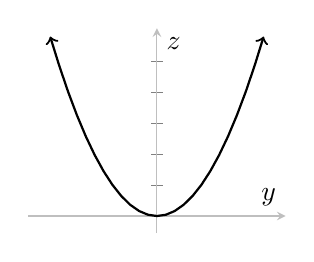
\begin{tikzpicture}
		\begin{axis}[
		xmin=-4.1,xmax=4.1,
		ymin=-1.1,ymax=12.1,
		xtick={0},
		ytick={2,4,6,8,10},
		yticklabels={},
		axis lines=middle,
		axis line style=lightgray,
		width=0.4\textwidth,
		xlabel={$y$},
		ylabel={$z$},
		]
		\addplot[black,style=thick,<->] expression[domain=-3.4:3.4,samples=25]{x^2}; 
		
		\end{axis}
		\end{tikzpicture}
		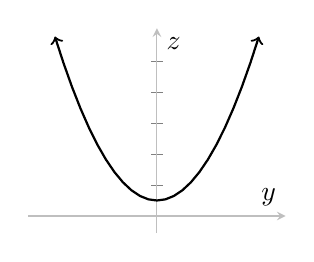
\begin{tikzpicture}
		\begin{axis}[
		xmin=-4.1,xmax=4.1,
		ymin=-1.1,ymax=12.1,
		xtick={0},
		ytick={2,4,6,8,10},
		yticklabels={},
		axis lines=middle,
		axis line style=lightgray,
		width=0.4\textwidth,
		xlabel={$y$},
		ylabel={$z$},
		]
		\addplot[black,style=thick,<->] expression[domain=-3.25:3.25,samples=25]{x^2+1}; 
		
		\end{axis}
		\end{tikzpicture}
		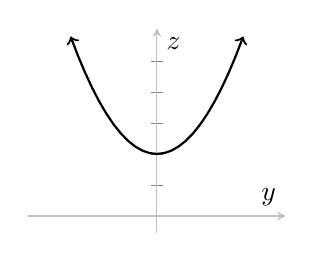
\begin{tikzpicture}
		\begin{axis}[
		xmin=-4.1,xmax=4.1,
		ymin=-1.1,ymax=12.1,
		xtick={0},
		ytick={2,4,6,8,10},
		yticklabels={},
		axis lines=middle,
		axis line style=lightgray,
		width=0.4\textwidth,
		xlabel={$y$},
		ylabel={$z$},
		]
		\addplot[black,style=thick,<->] expression[domain=-2.75:2.75,samples=25]{x^2+4}; 
		
		\end{axis}
		\end{tikzpicture}
	\end{center}
	\caption{Here are three vertical slices of the graph of the function $f(x,y) = x^2 + y^2$. From left to right, they are the $x = 0, x = 1$, and $x = 2$ slices, respectively.} \label{multi-introductory-example-slices}
\end{figure}

Slicing ``vertically in the other direction'' gives similar results. If we fix $y = 0$, we end up with the parabola $z = x^2$, and if we fix $y = 2$, we end up with the parabola $z = x^2 + 4$. 

It's also worth considering the ``level sets,'' ie, the ``horizontal'' slices of $\Gamma$ obtained by fixing various values of $z$. When $z = 0$, there is just the single point $x = y = 0$, ie, the origin. Fixing $z = 1$, the slice is given by $1 = x^2 +  y^2$, which is a circle of radius 1. Fixing $z = 17$, the slice is $17 = x^2 + y^2$, which is circle of radius $\sqrt{17}$. In fact, all of the level sets are circles, and these circles form a sort of ``topographic map'' style picture of the graph of $f$. See \cref{multi-introductory-example-level-sets}. 

\begin{figure}[ht]
	\begin{center}
		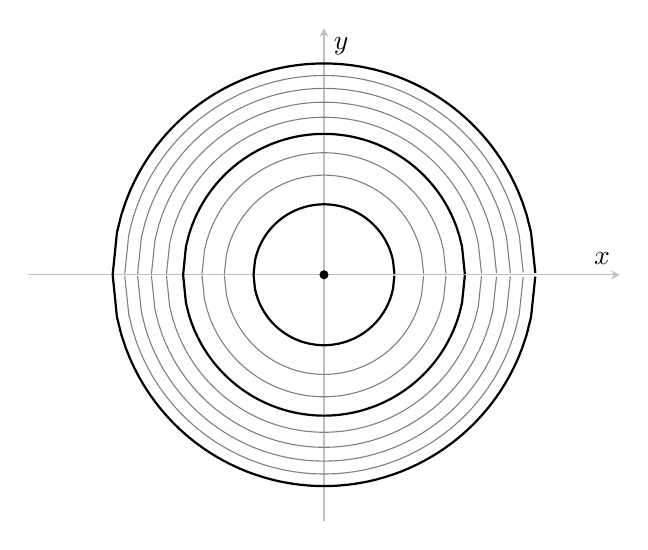
\begin{tikzpicture}
		\begin{axis}[
		xmin=-3.5,xmax=3.5,
		ymin=-3.5,ymax=3.5,
		xtick={0},
		ytick={0},
		xticklabels={},
		yticklabels={},
		axis lines=middle,
		axis line style=lightgray,
		width=0.75\textwidth,
		axis equal,
		xlabel={$x$},
		ylabel={$y$},
		]
		\node[color=black,draw=black,circle,fill,inner sep=1pt] at (axis cs:0,0) {};
		
		\addplot[black,style=thick,-] expression[domain=-1:1,samples=100]{sqrt(1-x^2)};
		\addplot[black,style=thick,-] expression[domain=-1:1,samples=100]{-sqrt(1-x^2)}; 
		
		\addplot[gray,-] expression[domain=-sqrt(2):sqrt(2),samples=100]{sqrt(2-x^2)};
		\addplot[gray,-] expression[domain=-sqrt(2):sqrt(2),samples=100]{-sqrt(2-x^2)}; 
		
		\addplot[gray,-] expression[domain=-sqrt(3):sqrt(3),samples=100]{sqrt(3-x^2)};
		\addplot[gray,-] expression[domain=-sqrt(3):sqrt(3),samples=100]{-sqrt(3-x^2)}; 
		
		\addplot[black,style=thick,-] expression[domain=-2:2,samples=100]{sqrt(4-x^2)};
		\addplot[black,style=thick,-] expression[domain=-2:2,samples=100]{-sqrt(4-x^2)}; 
		
		\addplot[gray,-] expression[domain=-sqrt(5):sqrt(5),samples=100]{sqrt(5-x^2)};
		\addplot[gray,-] expression[domain=-sqrt(5):sqrt(5),samples=100]{-sqrt(5-x^2)}; 
		
		\addplot[gray,-] expression[domain=-sqrt(6):sqrt(6),samples=100]{sqrt(6-x^2)};
		\addplot[gray,-] expression[domain=-sqrt(6):sqrt(6),samples=100]{-sqrt(6-x^2)}; 
		
		\addplot[gray,-] expression[domain=-sqrt(7):sqrt(7),samples=100]{sqrt(7-x^2)};
		\addplot[gray,-] expression[domain=-sqrt(7):sqrt(7),samples=100]{-sqrt(7-x^2)}; 
		
		\addplot[gray,-] expression[domain=-sqrt(8):sqrt(8),samples=100]{sqrt(8-x^2)};
		\addplot[gray,-] expression[domain=-sqrt(8):sqrt(8),samples=100]{-sqrt(8-x^2)}; 
		
		\addplot[black,style=thick,-] expression[domain=-3:3,samples=100]{sqrt(9-x^2)};
		\addplot[black,style=thick,-] expression[domain=-3:3,samples=100]{-sqrt(9-x^2)}; 
		 
		\end{axis}
		\end{tikzpicture}
	\end{center}
	\caption{Here is a ``topographic map'' style picture of the function $f(x,y) = x^2 + y^2$. Each circle is a level set of $f$. The innermost circle is the set of points such that $f(x,y) = 1$ (this is a circle of radius 1). The next circle from the inside (drawn in gray) is the set of points such that $f(x,y) = 2$ (this is a circle of radius $\sqrt{2}$). In general, the $k$th circle from the inside is the set of points such that $f(x,y) = k$. It is a circle of radius $\sqrt{k}$, and the circles where $\sqrt{k}$ is an integer are drawn in black rather than gray. The fact that the circles get ``closer together'' as $k$ increases is an indication that the function grows more and more rapidly as we get further from the origin. } \label{multi-introductory-example-level-sets}
\end{figure}


Stitching all of these two-dimensional slices together in our minds, we can see that the graph of $f$ is a ``big parabolic bowl'' inside $\R^3$. See \cref{multi-introductory-example-graph}. 

\begin{figure}[ht]
	\begin{center}
		\begin{tikzpicture}
		\begin{axis}[
		view={120}{15},
		axis lines=middle,
		xlabel={$x$},
		xtick={0},
		xmin=-3.1,xmax=3.1,
		ylabel={$y$},
		ytick={0},
		ymin=-3.1,ymax=3.1,
		zlabel={$z$},
		ztick={0},
		zmin=0,zmax=20,
		width=0.9\textwidth,
		]
		\addplot3[mesh,samples=50,domain=-3:3,colormap/Reds]{x^2+y^2}; 
		\end{axis}
		\end{tikzpicture}
	\end{center}
	\caption{The graph of the function  $f(x,y) = x^2 + y^2$. ``Vertical'' slices (ie, slices along planes that are parallel to either the $xz$-plane or the $yz$-plane) are parabolas. ``Horizontal slices'' (ie, slices along planes parallel to the $xy$-plane) are circles.} \label{multi-introductory-example-graph}
\end{figure}

\subsection*{Tangent plane at \texorpdfstring{$a = (2,1)$}{a = (2,1)}}

Now that we understand what the graph of $f$ looks like, let's try to figure out what the ``tangent plane'' $T$ at a point $a = (2,1)$ will look like. Of course, it's a plane inside $\R^3$ that passes through the point $(2, 1, f(2,1)) = (2, 1, 5)$. To specify which plane it actually is, we start by describing some lines that lie on this plane. 

Consider the $y = 1$ slice of $\Gamma$, which is a vertical slice containing the point $a$. We know that the graph of $\Gamma$ along this slice is the parabola $z = x^2 + 1$. So, slicing the tangent plane $T$ along $y = 1$ should yield the tangent line to this function of one variable, which we know how to compute from \cref{single}. The slope of this tangent line is
\[ \left.\frac{d }{d x} f(x, 1) \right|_{x = 2} = 4. \]
This quantity is called a \emph{partial derivative of $f$ at $a$}, and will be denoted $(\partial f/\partial x)(a)$.  Thus the tangent line is the line parametrized by
\[ h \mapsto \begin{bmatrix} 2 \\ 1 \\ 5 \end{bmatrix} + h \begin{bmatrix} 1 \\ 0 \\ 4 \end{bmatrix}. \]
The vector $(1,0,4)$ records the fact that the tangent line moves up 4 units in the $z$-direction for every 1 unit that it moves in $x$-direction. 

Similarly, we can consider the $x = 2$ slice, which is another vertical slice containing $a$. We know that the graph $\Gamma$ along this slice is the parabola $z = 4 + y^2$.The slope of the corresponding tangent line is
\[ \frac{\partial f}{\partial y}(a) = \left.\frac{d f(2, y)}{dy}\right|_{y = 1} = 2. \]
Thus this tangent line is the line parametrized by
\[ k \mapsto \begin{bmatrix} 2 \\ 1 \\ 5 \end{bmatrix} + k \begin{bmatrix} 0 \\ 1 \\ 2 \end{bmatrix}. \]
Again, the vector $(1,0,2)$ records the fact that the tangent line moves up 4 units in the $z$-direction for every 1 unit that it moves in $y$-direction. See \cref{multi-introductory-example-graph-tangent-lines}.

\begin{figure}[ht]
	\begin{center}
		\begin{tikzpicture}
		\begin{axis}[
		view={120}{15},
		axis lines=middle,
		xlabel={$x$},
		xtick={0},
		xmin=-3.1,xmax=3.1,
		ylabel={$y$},
		ytick={0},
		ymin=-3.1,ymax=3.1,
		zlabel={$z$},
		ztick={0},
		zmin=0,zmax=20,
		width=0.9\textwidth,
		axis line style=lightgray,
		]
		\addplot3[mesh,samples=50,domain=-3:3,colormap/Reds,opacity=0.25]{x^2+y^2}; 
		\node[color=black,draw=black,circle,fill,inner sep=2pt] at (axis cs:2,1,5) {};
		
		\addplot3[variable=t,domain=0:2,color=black,thick,->] (2+t,1,5+4*t);
		\addplot3[variable=t,domain=0:1,color=black] (2+t,1,5);
		\addplot3[variable=t,domain=0:1,color=black] (3,1,5+4*t);
		\node[color=black,draw=black,circle,fill,inner sep=0.5pt] at (axis cs:3,1,5) {};
		\node[color=black,draw=black,circle,fill,inner sep=0.5pt] at (axis cs:3,1,6) {};
		\node[color=black,draw=black,circle,fill,inner sep=0.5pt] at (axis cs:3,1,7) {};
		\node[color=black,draw=black,circle,fill,inner sep=0.5pt] at (axis cs:3,1,8) {};
		
		\addplot3[variable=t,domain=0:2,color=black,thick,->] (2,1+t,5+2*t);
		\addplot3[variable=t,domain=0:1,color=black] (2,1+t,5);
		\addplot3[variable=t,domain=0:1,color=black] (2,2,5+2*t);
		\node[color=black,draw=black,circle,fill,inner sep=0.5pt] at (axis cs:2,2,5) {};
		\node[color=black,draw=black,circle,fill,inner sep=0.5pt] at (axis cs:2,2,6) {};
		\end{axis}
		\end{tikzpicture}
	\end{center}
	\caption{The graph of the function  $f(x,y) = x^2 + y^2$, together with the point $(a, f(a)) = (2,1,5)$ and two of its tangent lines: one parallel to the $xz$-plane, and the other parallel to the $yz$-plane.} \label{multi-introductory-example-graph-tangent-lines}
\end{figure}

These two tangent lines uniquely determine the entire tangent plane $T$ (ie, $T$ is the plane containing these two lines). One description that falls out immediately from the parametrizations of the tangent lines we found above is that $T$ is the plane parametrized by
\[ \begin{bmatrix} h \\ k \end{bmatrix} \mapsto \begin{bmatrix} 2 \\ 1 \\ 5 \end{bmatrix} + h \begin{bmatrix} 1 \\ 0 \\ 4 \end{bmatrix} + k \begin{bmatrix} 0 \\ 1 \\ 2 \end{bmatrix} = \begin{bmatrix} 2 \\ 1 \\ 5 \end{bmatrix} + \begin{bmatrix} h \\ k \\ 4h + 2k \end{bmatrix}. \]
As we've seen, the important part of this expression is the bottom entry on the far right, the $4h + 2k$. The function $\R^2 \to \R$ given by $(h, k)  \mapsto 4h + 2k$ is what we will call the \emph{differential} or the \emph{total derivative} of $f$, and denote by $df_a$. Notice that $df_a$ is a linear map $\R^2 \to \R$. Moreover, its graph is a plane passing through the origin that is parallel to $T$. In other words, if we take the graph of $df_a$ and translate it over to the point $(2,1,5)$, we obtain exactly the tangent plane $T$. Speaking more loosely, $df_a$ records all of the ``slopey information'' about the tangent plane $T$. 

Notice moreover that, if $e_1, e_2$ are the standard basis vectors of $\R^2$ (cf. \cref{euclidean}), then
\[ \begin{aligned} df_a(e_1) &= 4 = \frac{\partial f}{\partial x}(a) \\
df_a(e_2) &= 2 = \frac{\partial f}{\partial y}(a) \end{aligned} \]
so the standard matrix representation $[df_a]$ (cf. \cref{matrix-representation-standard}) of the linear map $df_a$ is \begin{equation} \label{jacobian-matrix-example} [df_a] = \begin{bmatrix} 4 & 2 \end{bmatrix} = \begin{bmatrix} \dfrac{\partial f}{\partial x}(a) & \dfrac{\partial f}{\partial y}(a) \end{bmatrix}. \end{equation}

\subsection*{\texorpdfstring{$df_a$}{dfa} as an approximation}

Consider the function $r : \R^2 \to \R$ defined by
\[ (h,k) \mapsto f(a+(h,k))-f(a)-df_a(h,k).  \]
This is the multivariable analog of the single variable remainder function from \cref{remainder-linear}. Then
\[ r(h,k) = (2+h)^2 + (1+k)^2 - 5 - 4h - 2k = h^2 + k^2. \]
Notice that $r$ gets small rapidly as $(h,k) \to 0$. More precisely, the claim is that
\[ \lim_{(h,k) \to 0} \frac{|r(h,k)|}{|(h,k)|} = 0, \]
ie, that $|r(h,k)| = o(|(h,k)|)$ as $(h,k) \to 0$. 

In fact, for the claim, it doesn't matter whether $|-|$ denotes the euclidean norm or the max norm (cf. \cref{euclidean}). If it's the euclidean norm, we have
\[ \lim_{(h,k) \to 0} \frac{|r(h,k)|}{|(h,k)|_2} = \lim_{(h,k) \to 0} = \frac{h^2 + k^2}{\sqrt{h^2 + k^2}} = \lim_{(h,k) \to 0} \sqrt{h^2 + k^2} = 0. \]
If instead it's the max norm, observe that
\[ \frac{|r(h,k)|}{|(h,k)|_\infty} = \frac{h^2 + k^2}{|(h,k)|_\infty} \leq \frac{2(|(h,k)|_\infty)^2}{|(h,k)|_\infty} = 2|(h,k)|_\infty \]
so taking the limit as $(h,k) \to 0$ and applying the squeeze theorem yields the same result. 

Since $r$ gets small rapidly, we can say that the function $(h,k) \mapsto f(a) + df_a(h,k)$ is a good approximation of the function $(h,k) \mapsto f(a+(h,k))$ for small vectors $(h,k)$. Said differently, letting $x = a + (h,k)$, the function $x \mapsto f(a) + df_a(x-a)$ is a good approximation of $f$ near $a$. 

\subsection*{Overview}

In what follows, we will turn the above example on its head and \emph{define} the differential $df_a$ to be a linear function which yields a good approximation of $f$ near a point $a$, and then we will prove in \cref{jacobian-matrix} that partial derivatives (ie, derivatives along various ``slices'') can be used to compute the standard matrix representation of the the differential. This might seem a bit ``backwards'' given our analysis of the example above, but there is a good reason for doing this; it turns out that there are some bizarre functions where partial derivatives make sense, but tangent planes do not.

Much of the discussion below will involve arbitrary $m$ and $n$, which is impossible to visualize. However, the $m = 2, n = 1$ situation already captures most of the complexity that arises in the multivariable setting. If you run into something that you looks overly abstract because of the general $m$ and $n$, try to understand it when $m = 2, n = 1$. 

We'll be using a lot of linear algebra in this chapter. The notation $|-|$ will denote either the euclidean or the max norm on $\R^n$, and you can choose to interpret it to be whichever of the two norms you like better (in the calculation we did above, the euclidean norm was a little easier; but, in general, I find the max norm to be far more convenient). When it makes a difference which of the two norms on $\R^n$ we have in mind, we'll specify this explicitly.  We'll also need some facts about the operator norm as we go along; I encourage you to at least skim through \cref{operator-norm-basic} before proceeding. 

\section{Definition of the derivative}

Throughout, $S$ will denote a subset of $\R^m$. 

\begin{definition}[Differentiability at a point] \index{differentiable!differentiable at a point}
	A function $f : S \to \R^n$ is \emph{differentiable at} an interior point $a \in S$ if there exists a linear map $\ell : \R^m \to \R^n$ such that
	\[ |f(a+h)-f(a)-\ell(h)| = o(|h|) \text{ as } h \to 0. \]
\end{definition}

It turns out that there exists at most one linear map that has the above property. 

\begin{lemma} \label{differential-unique}
	Suppose $f : S \to \R^m$ is differentiable at an interior point $a \in S$. If $\ell$ and $\ell'$ are both linear maps $\R^m \to \R^n$ such that
	\[ |f(a+h) - f(a) - \ell(h)| = o(|h|) \text { and } |f(a+h) - f(a) - \ell'(h)| = o(|h|) \text{ as } h \to 0, \]
	then $\ell = \ell'$. 
\end{lemma}

\begin{proof}
	Let $\phi = \ell' - \ell$. Then $\phi$ is also a linear map $\R^m \to \R^n$. Moreover, observe that
	\[ \begin{aligned} |\phi(h)| &= |\ell'(h) - \ell(h)| \\
	&= |(f(a+h)-f(a)-\ell(h))-(f(a+h)-f(a)-\ell'(h)| \\
	&\leq |f(a+h)-f(a)-\ell(h)| + |f(a+h)-f(a)-\ell'(h)|. \end{aligned} \]
	Since both $|f(a+h)-f(a)-\ell(h)|$ and $|f(a+h)-f(a)-\ell'(h)|$ are $o(|h|)$, \cref{less-than-small-is-small,little-o-vector-space} imply that $|\phi(h)| = o(|h|)$ also. Then \cref{linear-and-small} implies that $\phi = 0$. 
\end{proof}

\begin{exercise}
	Look at the exercises from \cref{prelims} that are invoked in the proof above (namely, \cref{less-than-small-is-small,little-o-vector-space,operator-norm-is-norm}) and do any of them that you haven't already done.
\end{exercise}

\Cref{differential-unique} tells us that the following definition makes sense.  

\begin{definition} 
	Suppose $f : S \to \R^n$ is differentiable at an interior point $a \in S$. Then the \emph{differential} or the \emph{total derivative of $f$ at $a$}, denoted $df_a$, is the unique linear map $\R^m \to \R^n$ satisfying
	\[ |f(a+h)-f(a)-df_a(h)| = o(|h|) \text{ as } h \to 0.  \]
\end{definition}

\begin{pedanticremark}
	Since we're using $|-|$ to refer indiscriminately to both the euclidean and max norms, it might be worth pointing out that the above definition is independent of which norm you have in mind. More precisely, for any linear function $\ell : \R^m \to \R^n$, it is true that $|f(a+h)-f(a)-\ell(h)|_2 = o(|h|_2)$ if and only if $|f(a+h)-f(a)-\ell(h)|_\infty = o(|h|_\infty)$. You might try proving this if you're interested; the key is \cref{max-euclidean}. The upshot is that the differential $df_a$ is a ``good'' approximation for $f(a+h)-f(a)$, independently of whether we're measuring distances using the euclidean norm or the max norm. 
\end{pedanticremark}

This definition is fairly difficult to use in practice. Only a handful examples can be computed directly from the definition. Here are some that I think are instructive.

\begin{example}[Derivative of multiplication] \label{derivative-of-multiplication}
	Let $\mu : \R^2 \to \R$ be the multiplication map $\mu(x, y) = xy$. Let us show that 
	\[ d\mu_{(a,b)}(h, k) = bh + ak \]
	for all $(a,b) \in \R^2$ and $(h,k) \in \R^2$. Let $\ell(h,k) = bh + ak$. Observe that 
	\[ \mu((a,b)+(h,k)) - \mu(a,b) - \ell(h,k) = (a+h)(b+k) - ab - bh - ak = hk, \]
	and it is true that $|hk| = o(|(h,k)|)$. Roughly, this is because $|hk|$ is ``quadratic,'' which should be smaller than the ``linearish'' $|(h,k)|$. 
	
	To check that $|hk| = o(|(h,k)|)$ formally, we have to choose either the euclidean or the max norm. Let's use the max norm; if you prefer the euclidean norm, I'll leave the euclidean version of the following for you to check yourself. We have $|hk| \leq |(h,k)|_\infty^2$ by definition, so 
	\[ \frac{|hk|}{|(h,k)|_\infty} \leq \frac{|(h,k)|_\infty^2}{|(h,k)|_\infty} = |(h,k)|_\infty. \]
	The right hand side tends to 0 as $(h,k) \to 0$, so the squeeze theorem guarantees that the left hand side tends to as well. In other words, we have shown that 
	\[ |\mu((a,b)+(h,k)) - \mu(a,b) - \ell(h,k)| = |hk| = o(|(h,k)|_\infty), \]
	proving that $\ell = d\mu_{(a,b)}$. 
\end{example}

\begin{exercise}[Derivative of division] \label{derivative-of-division}
	Let $U = \{(x,y) \in \R^2 : y \neq 0\}$ and let $\Delta : U \to \R$ be the division map $\Delta(x, y) = x/y$. Show that 
	\[ d\Delta_{(a,b)}(h, k) = \frac{bh - ak}{b^2}. \]
	for all $(a, b) \in U$ and $(h,k) \in \R^2$. 
\end{exercise}

\begin{exercise}[``Linear maps are their own derivatives''] \label{derivative-of-linear}
	Suppose $\ell : \R^m \to \R^n$ is a linear map. Prove that $d\ell_a = \ell$ for all $a \in \R^m$.  
\end{exercise}

\begin{exercise} \label{derivative-of-line}
	Suppose $v, w \in \R^n$ and $f : \R \to \R^n$ is given by $f(t) = v + tw$. Calculate $df_a$ for any $a \in \R$. What is $df_a(1)$?
\end{exercise}

We will develop a bit more theory in order to compute more effectively. Meanwhile, we can prove the following directly from the definition. 

\begin{exercise} \label{differentiable-implies-continuous}
	If $f : S \to \R^n$ is differentiable at an interior point $a \in S$, show that $f$ must be continuous at $a$. 
\end{exercise}

Of course, the converse to \cref{differentiable-implies-continuous} is false. We've seen single variable examples; here are some multivariable examples. 

\begin{example}
	Consider the euclidean norm function $f : \R^2 \to \R$, given by 
	\[ f(x,y) = \sqrt{x^2 + y^2}. \]
	See \cref{euclidean-norm-graph}. This is definitely continuous at the origin, but the ``point'' of the cone at the origin suggests that this function is not differentiable at 0. Let's check this directly from the definition. 
	
	\begin{figure}[ht]
		\begin{center}
			\begin{tikzpicture}
			\begin{axis}[
			view={120}{15},
			axis lines=middle,
			xlabel={$x$},
			xtick={0},
			xmin=-5,xmax=5,
			ylabel={$y$},
			ytick={0},
			ymin=-5,ymax=5,
			zlabel={$z$},
			ztick={0},
			zmin=0,zmax=5,
			width=0.9\textwidth,
			]
			\addplot3[mesh, colormap/Reds, samples=50, domain=-3:3]{sqrt(x^2 + y^2)};
			\end{axis}
			\end{tikzpicture}
		\end{center}
		\caption{The graph of the function  $f(x,y) = \sqrt{x^2 + y^2}$ is an infinite cone, extending upwards, with its point at the origin.} \label{euclidean-norm-graph}
	\end{figure}
	
	Suppose for a contradiction that $f$ were differentiable at the origin. Then there would exist a linear map $\ell(h,k) = ah + bk$ such that $|f(h,k) - f(0) - \ell(h,k)| = o(|(h,k)|)$. 
	Observe that
	\[ |f(h,k) - f(0) - \ell(h,k)| = |\sqrt{h^2 +  k^2} - ah - bk|. \]
	Intuitively, notice that $\sqrt{h^2 + k^2}$ is ``linearish,'' and $ah + bk$ is definitely linear; so the difference should also be ``linearish,'' but the only way a ``linearish'' function can be $o(|(h,k)|)$ is if it's zero. But $\sqrt{h^2 + k^2}$ is not actually linear, so there cannot not exist $a$ and $b$ such that $\sqrt{h^2 + k^2} = ah + bk$. The conclusion of this intuitive argument is that it should be impossible for $|\sqrt{h^2 + k^2} - ah - bk|$ to be $o(|(h,k)|)$, no matter what $a$ and $b$ are. 
	
	More formally, we want to find a contradiction to the assertion that
	\[ \lim_{(h,k) \to 0} \frac{|\sqrt{h^2 + k^2} - ah - bk|}{|(h,k)|} = 0. \]
	If we approach the origin along the line $k = 0$, this says that
	\[ 0 = \lim_{h \to 0} \frac{|\sqrt{h^2} - ah|}{|h|} = \lim_{h \to 0} \left| \frac{|h|}{h} - a \right| \quad\implies\quad \lim_{h \to 0} \frac{|h|}{h} = a.  \]
	But this is nonsense, since $|h|/h$ does not converge at all as $h \to 0$. It tends to 1 as $h \to 0^+$ and to $-1$ as $h \to 0^-$. 
\end{example}

\begin{exercise} \label{continuous-not-differentiable}
	Consider the function $f : \R^2 \to \R$ given by \[ f(x,y) = \sqrt{|xy|}. \]
	See \cref{sqrt-x-y-graph}. Show that $f$ is continuous at the origin, but that it is not differentiable at the origin. 
	\begin{hint}
		If $f$ were differentiable at the origin, then there would exist $a, b \in \R$ such that 
		\[ \lim_{(h,k) \to 0} \frac{|f(h,k) - ah -  bk|}{|(h,k)|} = 0. \]
		Think about what happens with this limit when you approach the origin along the line $k = 0$, along the line $h = 0$, and along the line $h = k$.
	\end{hint}
	\begin{figure}[ht]
		\begin{center}
			\begin{tikzpicture}
			\begin{axis}[
			view={120}{15},
			axis lines=middle,
			xlabel={$x$},
			xtick={0},
			xmin=-5,xmax=5,
			ylabel={$y$},
			ytick={0},
			ymin=-5,ymax=5,
			zlabel={$z$},
			ztick={0},
			zmin=0,zmax=5,
			width=0.9\textwidth,
			]
			\addplot3[mesh, colormap/Reds, samples=50, domain=-4:4]{sqrt(abs(x*y))};
			\end{axis}
			\end{tikzpicture}
		\end{center}
		\caption{The graph of the function  $f(x,y) = \sqrt{|xy|}$. The graph has four ``leaves,'' which look a bit like the ``leaves'' of the Sydney Opera House, or of the Lotus Temple in New Delhi.} \label{sqrt-x-y-graph}
	\end{figure}
\end{exercise}

\begin{exercise} \label{differentiable-at-a-point-but-not-in-any-neighborhood}
	Describe the set of all points $(a, b) \in \R^2$ where the function $f : \R^2 \to \R$ given by \[ f(x,y) = |xy| \] is not differentiable. 
\end{exercise}

\section{Computing derivatives}

\subsection{Sum and scalar multiples rule} 

\begin{exercise}[Sum rule] \label{sum-rule} \index{sum rule}
	Prove that, if $f, g : S \to \R^n$ are both differentiable at an interior point $a \in S$, then $f + g$ is also differentiable at $a$ and \[ d(f+g)_a = df_a + dg_a. \]
\end{exercise}

\begin{solution}{\cref{sum-rule}}
	Observe that 
	\[ |(f+g)(a+h)-(f+g)(a)-(df_a+dg_a)(h)| = |f(a+h) - f(a) - df_a(h) + g(a+h) - g(a) - dg_a(h)| \leq |f(a+h) - f(a) - df_a(h)| + |g(a+h) - g(a) - dg_a(h)|. \]
	Both $|f(a+h) - f(a) - df_a(h)|$ and $|g(a+h) - g(a) - dg_a(h)|$ are $o(|h|)$ by definition of the derivative, so it follows from \cref{little-o-vector-space,less-than-small-is-small} that $|(f+g)(a+h)-(f+g)(a)-(df_a+dg_a)(h)|$ is $o(|h|)$. Thus $df_a + dg_a = d(f+g)_a$. 
\end{solution}

\begin{exercise}[Scalar multiples rule] \label{scalar-multiples-rule} \index{scalar multiples rule}
	Prove that, if $c$ is a constant and $f : S \to \R^n$ is differentiable at an interior point $a \in S$, then $cf$ is also differentiable at $a$ and \[ d(cf)_a = c \cdot df_a. \]
\end{exercise}

\subsection{Chain rule}

The proof of the following is essentially the same as the second proof of the single variable chain rule given in \cref{chain-rule-single-section}. Since this proof is basically a repeat, some details are omitted; you are asked to fill in the details in \cref{chain-rule-details} below. 

\begin{theorem}[Chain rule] \label{chain-rule} \index{chain rule}
	Suppose that $S$ and $T$ are subsets of $\R^m$ and $\R^n$, respectively, that $f : S \to \R^n$ is differentiable at an interior point $a$, that $f(S) \subseteq T$ and $f(a)$ is an interior point of $T$, and that $g : T \to \R^p$ is differentiable at $f(a)$. Then the composite $g \circ f : S \to \R^p$ is also differentiable at $a$, and 
	\[ d(g \circ f)_a = dg_{f(a)} \circ df_a. \]
\end{theorem}

\begin{proof}
	Define the ``error in approximation'' functions\index{error in approximation function@``error in approximation'' function}
	\[ \begin{aligned} 
	r(h) &= f(a+h)-f(a) - df_a(h) \\ 
	s(k) &= g(f(a)+k)-g(f(a))-dg_{f(a)}(k) 
	\end{aligned} \]
	and then observe that
	\begin{equation} \label{rewrite-error} g(f(a+h)) - g(f(a)) - dg_{f(a)}(df_a(h)) = dg_{f(a)}(r(h)) + s(df_a(h)+r(h)). \end{equation}
	This means that 
	\[ |g(f(a+h)) - g(f(a)) - dg_{f(a)}(df_a(h))| \leq |dg_{f(a)}(r(h))| + |s(df_a(h)+r(h))|. \]
	Since $dg_{f(a)}$ is linear and $|r(h)| = o(|h|)$, \cref{chain-rule-details} guarantees that $|dg_{f(a)}(r(h))| = o(|h|)$ also. Thus, by \cref{little-o-vector-space}, it is sufficient to prove that $|s(df_a(h) + r(h))| = o(|h|)$. To do this, define $\eta(k) = |s(k)|/|k|$ and then notice that 
	\[ \begin{aligned} \frac{|s(df_a(h)+r(h))|}{|h|} &= \eta(df_a(h)+r(h)) \cdot \frac{|df_a(h) + r(h)|}{|h|} \\
	&\leq \eta(df_a(h) + r(h)) \left( \|df_a\| + \frac{|r(h)|}{|h|} \right) \end{aligned} \]
	where we have used \cref{operator-norm-reformulation} for the inequality.
	We now take the limit as $h \to 0$. Using the facts that $\eta \circ (df_a + r)$ is continuous at 0 and that $|r(h)| = o(|h|)$, we obtain the result. 
\end{proof}

\begin{exercise} \label{chain-rule-details}
	\begin{enumerate}[(a)]
		\item Prove \cref{rewrite-error}. 
		
		\item Do \cref{operator-norm-reformulation} if you haven't already. 
		
		\item \label{linear-of-small-is-small} Suppose $r : \R^m \to \R^n$ is a function such that $|r(h)| = o(|h|)$ as $h \to 0$. If $\ell : \R^n \to \R^p$ is linear, prove that $|\ell(r(h))| = o(|h|)$ also.
		
		\begin{hint} Even though the operator norm\index{operator norm} does not appear anywhere in the statement of this exercise, you might find the concept useful (especially \cref{operator-norm-reformulation}). 
		\end{hint}
		
		\item Prove that $\eta \circ (df_a + r)$ is continuous at 0. 
	\end{enumerate}
\end{exercise}

\begin{comment}
\begin{proof}
Observe that
\[ \frac{|\ell(r(v))|}{|v|} \leq \frac{\|\ell\| \cdot |r(v)|}{|v|}. \]
Since $|r(v)| = o(|v|)$, we see that the right-hand side tends to 0 as $v \to 0$. The squeeze theorem thus guarantees that $|\ell(r(v))| = o(|v|)$ also. 
\end{proof}
\end{comment}

\subsection{Differentiability by components}

Recall that we asserted at the beginning of this chapter that the ``multi'' in the name of this chapter refers to the number of inputs (rather than the number of outputs). This section is where we show that understanding the $n = 1$ case is ``enough'' to understand general $n$.

\begin{definition}[Component functions] \index{component function}
	For any function $f : S \to \R^n$, we define the $j$th \emph{component function} $f_j : S \to \R$ to be the composite $\pi_j \circ f$, where $\pi_j$ is the $j$th projection map (cf. \cref{euclidean}).\index{projection map}
\end{definition}

\begin{proposition} \label{differentiable-by-components}
	A function $f : S \to \R^n$ is differentiable at an interior point $a \in S$ if and only if the component function $f_j : S \to \R$ is differentiable at $a$ for all $j = 1, \dotsc n$. Moreover,
	\begin{equation} \label{derivative-of-components} df_a(h) = \begin{bmatrix} df_{1,a}(h) \\ \vdots \\ df_{n,a}(h) \end{bmatrix}. \end{equation}
\end{proposition}

\begin{proof}
	If $f$ is differentiable at $a$, then the composite $f_j = \pi_j \circ f$ is also differentiable at $a$ by the chain rule \ref{chain-rule}. Moreover, since $\pi_j$ is linear, we know that $d\pi_{j,f(a)} = \pi_j$ by \cref{derivative-of-linear}. Thus, by the chain rule, 
	\[ df_{j,a}(h) = (d\pi_{j,f(a)} \circ df_a)(h) = \pi_j(df_a(h)) \]
	for all $j$, which is precisely \cref{derivative-of-components}. 
	For the converse, we turn \cref{derivative-of-components} on its head. Suppose $f_j$ is differentiable at $a$ for all $j$, and let $\ell : \R^m \to \R^n$ be the linear map 
	\[ \ell(h) = \begin{bmatrix} df_{1,a}(h) \\ \vdots \\ df_{n,a}(h) \end{bmatrix}.  \]
	We now want to show that $|f(a+h)-f(a)-\ell(h)| = o(|h|)$ as $h \to 0$. Observe that the component functions of $h \mapsto f(a+h)-f(a)-\ell(h)$ are given by
	\[ v \mapsto \pi_j \left( f(a+h)-f(a)-\ell(h) \right) = f_j(a+h)-f_j(a)-df_{j,a}(h) \]
	since $\pi_j$ is linear, 
	and we know that $|f_j(a+h)-f_j(a)-df_{j,a}(h)| = o(|h|)$. By \cref{components-are-small-implies-small} below applied with the function $r(h) = f(a+h)-f(a)-\ell(h)$, we conclude that $|f(a+h)-f(a)-\ell(h)| = o(|h|)$. 
\end{proof}

\begin{exercise} \label{components-are-small-implies-small}
	Show that if $S$ is a neighborhood of 0 in $\R^m$ and $r :  S  \to \R^n$ is a function such that $|r_j(h)| = o(|h|)$ as $h \to 0$ for all $j = 1, \dotsc, n$, then $|r(h)| = o(|h|)$ also.
	\begin{hint}
		This is easy if you're using the max norm. If you're using the euclidean norm, you may find it useful to do \cref{max-euclidean} first. 
	\end{hint}
\end{exercise}

\begin{exercise}
	Suppose $S$ is a subset of $\R$ and $f : S \to \R^n$ is differentiable at an interior point $a$. Show that the standard matrix representation $[df_a]$ of the linear map $df_a : \R \to \R^nn$ is given by 
	\[ [df_a] = \begin{bmatrix} f_1'(a) \\ \vdots \\ f_n'(a) \end{bmatrix}, \]
	where $f_j'(a)$ is the derivative of the single variable function $f_j : S \to \R$ in the sense of \cref{single}. 
\end{exercise}

\subsection{Product and quotient rules}

We showed in the previous section that it's enough to understand the $n = 1$ case, ie, the case of real-valued (rather than $\R^n$-valued) functions. So in this section and the next, we'll focus our attention on real-valued functions. 

Note that we can combine real-valued functions in more ways than the ones we've already discussed; specifically, we can multiply and divide them. As in \cref{single}, we have product and quotient rules to deal with this. As it turns out, we can actually derive these using the multivariable chain rule \ref{chain-rule}!

\begin{proposition}[Product rule] \label{product-rule} \index{product rule}
	Suppose $f, g : S \to \R$ are both differentiable at an interior point $a \in S$. Then $fg$ is also differentiable at $a$ and
	\[ d(fg)_a = g(a)df_a + f(a) dg_a. \]
\end{proposition}

\begin{proof}
	Let $f \times g$ denote the function $S \to \R^2$ defined by
	\[ (f \times g)(x) = (f(x), g(x)). \]
	Observe that the first and second component functions of $f \times g$ are $f$ and $g$, respectively; thus it follows from \cref{differentiable-by-components} that 
	\[ d(f \times g)_a(h) = (df_a(h), dg_a(h)). \]
	Let $\mu : \R^2 \to \R$ denote the multiplication map $\mu(x,y) = xy$ that we considered in \cref{derivative-of-multiplication}. Then $fg = \mu \circ (f \times g)$, so by the chain rule \ref{chain-rule}, we have that 
	\[ \begin{aligned} d(fg)_a(h) &= d\mu_{(f(a),g(a))}(d(f \times g)_a(h)) \\
	&= d\mu_{f(a),g(a)}(df_a(h), dg_a(h)) \\
	&= g(a) df_a(h) + f(a)dg_a(h), \end{aligned} \]
	where we have used the calculation from \cref{derivative-of-multiplication} for the final step. 
\end{proof}

\begin{exercise} \label{reciprocal-rule}
	Suppose $f : S \to \R$ is differentiable at an interior point $a \in S$ and that $f(a) \neq 0$. Show that $1/f$ is also differentiable at $a$, and
	\[ d(1/f)_a = -\frac{df_a}{f(a)^2}.  \]
	\begin{hint}
		Consider the function $\iota : \R \setminus \{0\} \to \R$ given by $\iota(x) = 1/x$. This is a single variable function, so we know $d\iota_x$ from \cref{single}. Now note that $1/f = \iota \circ f$. 
	\end{hint}
\end{exercise}

\begin{exercise}[Quotient rule] \label{quotient-rule} \index{quotient rule}
	Suppose $f, g : S \to \R$ is differentiable at an interior point $a \in S$ and that $g(a) \neq 0$. Show that $f/g$ is also differentiable at $a$, and that
	\[ d(f/g)_a = \frac{g(a)df_a - f(a)dg_a}{g(a)^2}. \]
	\begin{hint}
		One approach is to combine \cref{reciprocal-rule} and the product rule \ref{product-rule}. An alternative approach is to mimic the proof of the product rule \ref{product-rule} (using the division function of \cref{derivative-of-division} in place of the multiplication function of  \cref{derivative-of-multiplication}). 
	\end{hint}
\end{exercise}

\subsection{Directional and partial derivatives}

We now formalize the ``slicing'' we did in \cref{multi-introductory-example}. 

\begin{definition}[Directional derivatives] \index{directional derivative} \index{partial derivative}
	Suppose $f : S \to \R$ is a function, $a \in S$ is an interior point, and $h \in \R^m$ is a vector. The \emph{directional derivative of $f$ at $a$ with respect to $h$}, denoted $\partial_h f(a)$, is defined to be the limit
	\[ \lim_{t \to 0} \frac{f(a+th) - f(a)}{t}. \]
	If $h = e_i$ is the $i$th standard basis vector (cf. \cref{euclidean}), then this is called the \emph{$i$th partial derivative of $f$ at $a$} and denoted $\partial_i f(a)$ (instead of $\partial_{e_i} f(a)$). If we're using $x_i$ to denote the $i$th component of the input of $f$, then $\partial_i f(a)$ is sometimes also denoted by one of the following. 
	\[ f_{x_i}(a) \quad \left. \frac{\partial f}{\partial x_i}\right|_{x = a} \quad \left.\frac{\partial}{\partial x_i} f(x)\right|_{x = a} \quad \frac{\partial f}{\partial x_i}(a) \]
\end{definition}

You may remember from multivariable calculus that partial derivatives behave a great deal like single variable derivatives. The reason for this is the following important remark, which reinterprets a directional derivative as a single variable derivative. 

\begin{remark} \label{directional-to-single}
	For $a \in S$ an interior point and $h \in \R^m$, consider the function $\xi : \R \to \R^m$ given by $\xi(t) = a + th$. This is the ``line through $a$ in the direction of the vector $h$.'' Note that $0 = \xi^{-1}(a)$ is an interior point of $\xi^{-1}(S)$ since $a$ is a interior point of $S$. If $f : S \to \R$ is a function, then $f \circ \xi$ is a single variable function $\xi^{-1}(S) \to \R$, and we have
	\[ \partial_h f(a) = (f \circ \xi)'(0), \]
	just by writing out the definition of both sides. A bit more geometrically, $f \circ \xi$ can be thought of as the restriction of $f$ to the line passing through $a$ in the direction of $h$. This is a single variable function, and the derivative of this single variable function at 0 is the directional derivative of $f$ at $a$ with respect to $h$. 
\end{remark}

\begin{example} \label{computing-partials-example}
	Consider the function $f : \R^2 \to \R$ given by $f(x, y) = \sin(xy^2)$. Fix $(a, b) \in \R^2$ and define $\xi : \R \to \R^2$ by $\xi(t) = (a + t, b)$. In other words, $\xi$ is the line through $(a, b)$ in the direction of the vector $(1,0)$, as in \cref{directional-to-single}. Then
	\[ (f \circ \xi)(t) = f(a + t, b) = \sin((a+t)b^2).  \]
	Then
	\[ \begin{aligned} \frac{\partial f}{\partial x}(a, b) &= (f \circ \xi)'(0) \\
	&= \left.\frac{d}{dt} \left(\sin((a+t)b^2) \right) \right|_{t = 0} \\
	&= \left. b^2\cos((a+t)b^2)\right|_{t = 0} \\
	&= b^2\cos(ab^2). \end{aligned}  \]
\end{example}

\begin{exercise}
	With notation as in \cref{computing-partials-example}, compute $(\partial f/\partial y)(a, b)$. 
\end{exercise}

\begin{exercise} \label{basic-directional-derivative-properties}
	Suppose $f : S \to \R$ is a function and $a \in S$ is an interior point. Prove the following. 
	\begin{enumerate}[(a)]
		\item $\partial_0 f(a) = 0$.  
		\item If $\partial_h f(a)$ exists for some $h \in \R^m$, then $\partial_{\lambda h} f(a)$ also exists for all $\lambda \in \R$ and \[ \partial_{\lambda h} f(a) = \lambda \partial_h f(a). \] 
	\end{enumerate}
\end{exercise}

We can use \cref{directional-to-single} to prove some directional derivative analogs of results we proved in \cref{single}.

\begin{exercise}[Product rule for directional derivatives] \label{product-rule-directional} \index{product rule}
	Suppose $f, g : S \to \R$ are functions, $a \in S$ is an interior point, and $h \in \R^m$ is a vector such that $\partial_h f(a)$ and $\partial_h g(a)$ both exist. Prove that $\partial_h (fg)(a)$ also exists and that
	\[ \partial_h (fg)(a) = g(a)\partial_h(f)(a) + f(a) \partial_h g(a). \]
	\begin{hint} 
		Use \cref{directional-to-single} and the single variable product rule \ref{product-rule-single}.
	\end{hint}
\end{exercise}

\begin{exercise}[Quotient rule for directional derivatives] \label{quotient-rule-directional} \index{quotient rule}
	Suppose $f, g : S \to \R$ are functions, $a \in S$ is an interior point such that $g(a) \neq 0$ and $\partial_h f(a)$ and $\partial_h g(a)$ both exist for some $h \in \R^m$. Show that $\partial_h(f/g)(a)$ also exists and 
	\[ \partial_h(f/g)(a) = \frac{g(a)\partial_h f(a) - f(a)\partial_h g(a)}{g(a)^2}. \]
	\begin{hint} Use \cref{directional-to-single} and the single variable quotient rule \ref{quotient-rule-single}. \end{hint} 
\end{exercise}

\begin{exercise}[Interior extremum theorem for directional derivatives] \label{interior-extremum-directional} \index{extremum!interior extremum theorem}
	Suppose $f : S \to \R$ is a function and an interior point $a \in S$ is a local extremum of $f$. Show that, if $\partial_h f(a)$ exists for some $h \in \R^m$, then $\partial_h f(a) = 0$. 
	\begin{hint} Use \cref{directional-to-single} and the single variable interior extremum theorem \ref{interior-extremum}. \end{hint}
\end{exercise}

Just as the converse to the single variable interior extremum theorem \ref{interior-extremum} is false (cf. \cref{interior-extremum-converse-false}), so too is the converse to the interior extremum theorem for directional derivatives \ref{interior-extremum-directional}, except that there are now even more ways for the converse to fail. Here are some examples to illustrate this.  

\begin{example} \label{saddle}
	Consider the function $f : \R^2 \to \R$ given by \[ f(x, y) = x^2 - y^2. \]
	Let $\xi(t) = 0 + te_1 = (t, 0)$. Then $f \circ \xi$ has a minimum at 0, so $(f \circ \xi)'(0) = (\partial f)/(\partial x)(0) = 0$. Similarly, if $\xi(t) = 0 + te_2 = (0, t)$, then $f \circ \xi$ has a maximum at 0, so $(f \circ \xi)'(0) = (\partial f)/(\partial y)(0) = 0$ also. But clearly these two facts together mean that 0 cannot be a local extremum of $f$. See \cref{saddle-graph}. This kind of a point is sometimes called a ``saddle.''\index{saddle}
	\begin{figure}[ht]
		\begin{center}
			\begin{tikzpicture}
			\begin{axis}[
			view={120}{15},
			axis lines=middle,
			xlabel={$x$},
			xtick={0},
			xmin=-5,xmax=5,
			ylabel={$y$},
			ytick={0},
			ymin=-5,ymax=5,
			zlabel={$z$},
			ztick={0},
			zmin=-20,zmax=20,
			width=0.9\textwidth,
			]
			\addplot3[mesh,samples=50,domain=-4:4,
			colormap/Reds]{x^2-y^2};
			\end{axis}
			\end{tikzpicture}
		\end{center}
		\caption{The graph of the function  $f(x,y) = x^2 - y^2$. Vertical slices along planes parallel to the $xz$-plane are downwards facing parabolas, while those along planes parallel to the $yz$-plane are upwards facing parabolas.} \label{saddle-graph}
	\end{figure}
\end{example}

\begin{exercise} \label{all-directionals-vanish-but-not-extremum}
	Consider the function $f : \R^2 \to \R$ given by 
	\[ f(x, y) = (y- x^2)(y - 3x^2). \]
	See \cref{all-directionals-vanish-but-not-extremum-graph} for the graph of $f$. 
	\begin{figure}[ht]
		\begin{center}
			\begin{tikzpicture}
			\begin{axis}[
			view={120}{15},
			axis lines=middle,
			xlabel={$x$},
			xtick={0},
			xmin=-1,xmax=1,
			ylabel={$y$},
			ytick={0},
			ymin=-1,ymax=1,
			zlabel={$z$},
			ztick={0},
			zmin=-2,zmax=10,
			width=0.9\textwidth,
			]
			\addplot3[mesh,samples=50,domain=-1:1,
			colormap/Reds]{(y- x^2)*(y - 3*x^2)};
			\end{axis}
			\end{tikzpicture}
		\end{center}
		\caption{The graph of the function  $f(x,y) = (y- x^2)(y - 3x^2)$.} \label{all-directionals-vanish-but-not-extremum-graph}
	\end{figure}
	\begin{enumerate}[(a)]
		\item Show that the origin is \emph{not} a local extremum of $f$. \begin{hint} Consider the values of $f$ on points of the form $(0,b)$ and $(a, 2a^2)$ near the origin. You might consider identifying where these points are on the graph depicted in \cref{all-directionals-vanish-but-not-extremum-graph} to get a more visual sense of what's going on. \end{hint}
		\item Show that $f$ has a local minimum when restricted to an arbitrary line through the origin. Conclude that $\partial_h f(a) = 0$ for all $h \in \R^2$. 
	\end{enumerate}
\end{exercise}

\begin{exercise}
	Consider the function $f : \R^2 \to \R$ given by
	\[ f(x,y) = 2x^3 - 3x^2 + 2y^3 + 3y^2. \]
	Find all points $a \in \R^2$ such that $\partial_1 f(a) = \partial_2 f(a) = 0$. Of these points, which (if any) are local extremums? 
\end{exercise}

Now for the main result of this section, which relates the differential to directional derivatives. Note that we will generalize this result slightly in \cref{jacobian-matrix} below. 

\begin{proposition} \label{differentiable-implies-directionals}
	If $f : S \to \R$ is differentiable at an interior point $a \in S$ and $h \in \R^m$, then \[ df_a(h) = \partial_h f(a). \]
	Thus, the standard matrix representation $[df_a]$ of the total derivative $df_a : \R^m \to \R$ is a $1 \times m$ matrix whose $i$th entry is the $i$th partial derivative $\partial_i f(a)$. 
	\[ [df_a] = \begin{bmatrix} \partial_1 f(a) & \partial_2 f(a) & \dotsb & \partial_m f(a) \end{bmatrix} \]
\end{proposition}

\begin{proof}
	If $h = 0$, we know that $\partial_0 f(a) = 0$ by \cref{basic-directional-derivative-properties} and that $df_a(0) = 0$ since $df_a$ is linear, so we are done. Thus we can assume that $h$ is nonzero. Let $r$ be the ``error in approximation'' function
	\[ r(k) = f(a+k) - f(a) - df_a(k), \]
	so that $|r(k)| = o(|k|)$ as $k \to 0$. Letting $k = th$, we see that
	\[ r(th) = f(a+th) - f(a) - df_a(th) = f(a+th) - f(a) - t df_a(h) \]
	by linearity of $df_a$, so
	\[ \frac{r(th)}{t} = \frac{f(a+th) - f(a) - tdf_a(h)}{t} = \frac{f(a+th) - f(a)}{t} - df_a(h). \]
	Then 
	\[\lim_{t \to 0} \left| \frac{f(a+th) - f(a)}{t} - df_a(h) \right| 
	= \lim_{t \to 0} \frac{|r(th)|}{|t|} = \lim_{t \to 0} \frac{|r(th)|}{|th|} \cdot |h| = 0 \]
	where we used the fact that $|r(k)| = o(|k|)$ as $k \to 0$ for the last step. This tells us that $\partial_h f(a)$ exists and equals $df_a(h)$. In particular, applying this with $h = e_i$, we see that $df_a(e_i) = \partial_i f(a)$, which yields the standard matrix representation.  
\end{proof}

\begin{remark} \label{gradient}
	If $f : S \to \R$ is differentiable at an interior point $a \in S$, the column vector \[ [df_a]^T = \begin{bmatrix} \partial_1 f(a) \\ \partial_2 f(a) \\ \vdots \\ \partial_m f(a) \end{bmatrix} \in \R^m \]
	is often called the \emph{gradient}\index{gradient}  of $f$ at $a$, and is denoted $\nabla f(a)$. If $h \in \R^m$ is any vector, then 
	\[ [df_a(h)] = [df_a]h = [df_a]^T \cdot h = \nabla f(a) \cdot h, \]
	where the $\cdot$ denotes the dot product. 
\end{remark}

Now for the important caveat: unfortunately, the converse to \cref{differentiable-implies-directionals} is \emph{not} true: the existence of all partial derivatives is not sufficient to guarantee differentiability. Even the existence of all \emph{directional} derivatives is not sufficient to guarantee differentiability. In fact, we cannot guarantee differentiability even if all directional derivatives exist \emph{and} the function $h \mapsto \partial_h f(a)$ is linear. 

Here are several examples to drive home these points. They're useful examples to study closely; you'll gain valuable intuition about multivariable differentiability and the somewhat subtle way in which it is related to single variable differentiability. 

\begin{exercise}
	Consider the function $f : \R^2 \to \R$ defined as follows. 
	\[ f(x, y) = \begin{cases} 1 &  \text{if } x = 0 \text{ or } y = 0 \\ 0 & \text{otherwise} \end{cases} \]
	\begin{enumerate}[(a)]
		\item Sketch a graph of $f$ by hand. 
		\item Show that $f$ is discontinuous (so it cannot be differentiable, by \cref{differentiable-implies-continuous}). 
		\item Show that both partial derivatives of $f$ exist at the origin. 
	\end{enumerate}
\end{exercise}

\begin{exercise} \label{partials-dont-imply-differentiable}
	Consider the function $f : \R^2 \to \R$ defined as follows.
	\[ f(x, y) = \begin{cases} \dfrac{x y}{x^2 + y^2} &  \text{if } (x, y) \neq 0 \\ 0 & \text{if } (x, y) = 0 \end{cases} \]
	See \cref{partials-dont-imply-differentiable-graph}. Clearly $f$ is continuous (and differentiable) away from the origin.
	\begin{enumerate}[(a)]
		\item Show that $f$ is discontinuous at the origin (so it cannot be differentiable, by \cref{differentiable-implies-continuous}). 
		\item Show that both partial derivatives of $f$ exist at the origin. 
	\end{enumerate} 
	\begin{figure}[ht]
		\begin{center}
			\begin{tikzpicture}
			\begin{axis}[
			view={120}{15},
			axis lines=middle,
			axis line style=black,
			xlabel={$x$},
			xtick={0},
			xmin=-1,xmax=1,
			ylabel={$y$},
			ytick={0},
			ymin=-1,ymax=1,
			zlabel={$z$},
			ztick={0},
			zmin=-0.5,zmax=0.75,
			width=0.6\textwidth,
			]
			\addplot3[mesh,samples=50,domain=-1:1,
			colormap/Reds,opacity=0.5]{x*y/(x^2+y^2)};
			\end{axis}
			\end{tikzpicture}
			\begin{tikzpicture}
			\begin{axis}[
			view={60}{15},
			axis lines=middle,
			axis line style=black,
			xlabel={$x$},
			xtick={0},
			xmin=-1,xmax=1,
			ylabel={$y$},
			ytick={0},
			ymin=-1,ymax=1,
			zlabel={$z$},
			ztick={0},
			zmin=-0.5,zmax=0.75,
			width=0.6\textwidth,
			]
			\addplot3[mesh,samples=50,domain=-1:1,
			colormap/Reds,opacity=0.5]{x*y/(x^2+y^2)};
			\end{axis}
			\end{tikzpicture}
		\end{center}
		\caption{Two views of the graph of the function $f$ from \cref{partials-dont-imply-differentiable}. The one on the left is obtained from the one on the right by a 90$^\circ$ rotation counterclockwise around the $z$-axis.} \label{partials-dont-imply-differentiable-graph}
	\end{figure}
\end{exercise}

\begin{exercise} \label{directionals-dont-imply-differentiable}
	Consider the function $f : \R^2 \to \R$ given by
	\[ f(x,y) = \begin{cases} \dfrac{x^3}{x^2 +y^2} & \text{if } (x, y) \neq 0 \\ 0 & \text{if } (x,y) = 0. \end{cases} \]
	See \cref{directionals-dont-imply-differentiable-graph}.
	\begin{figure}[ht]
		\begin{center}
			\begin{tikzpicture}
			\begin{axis}[
			view={120}{15},
			axis lines=middle,
			xlabel={$x$},
			xtick={0},
			xmin=-1,xmax=1,
			ylabel={$y$},
			ytick={0},
			ymin=-1,ymax=1,
			zlabel={$z$},
			ztick={0},
			zmin=-0.5,zmax=0.75,
			width=0.9\textwidth,
			]
			\addplot3[mesh,samples=50,domain=-1:1,
			colormap/Reds]{x^3/(x^2+y^2)};
			\end{axis}
			\end{tikzpicture}
		\end{center}
		\caption{The graph of the function  $f$ from \cref{directionals-dont-imply-differentiable}.} \label{directionals-dont-imply-differentiable-graph}
	\end{figure} 
	\begin{enumerate}[(a)]
		\item Show that $f$ is continuous. 
		\item Show that $\partial_{(h,k)} f(0)$ exists for all nonzero $(h,k) \in \R^2$, but that $f$ is not differentiable at the origin.
		\begin{hint}
			Calculate a formula for $\partial_{(h,k)} f(0)$ for all $(h,k) \in \R^2$, and show that the function $\R^2 \to \R$ given by $(h,k) \mapsto \partial_{(h,k)} f(0)$ is not linear. Explain why \cref{differentiable-implies-directionals} then implies that $f$ is \emph{not} differentiable at 0.  
		\end{hint}
		\item Suppose that $\gamma : \R \to \R^2$ is differentiable at 0, that $\gamma(0) = 0$, and that $d\gamma_0 \neq 0$. Show that $f \circ \gamma$ is differentiable at 0. 
	\end{enumerate} 
\end{exercise}

\begin{exercise} \label{directionals-and-linear-dont-imply-differentiable}
	Consider the function $f : \R^2 \to \R$ given by
	\[ f(x,y) = \begin{cases} |x| & \text{if } y = x^2 \\ 0 & \text{otherwise}. \end{cases} \]
	\begin{enumerate}[(a)]
		\item Sketch a graph of $f$ by hand.
		\item Show that $f$ is continuous at the origin. 
		\item Show that all directional derivatives of $f$ at the origin exist and are equal to 0. 
		\begin{hint}
			First show it for the partial derivatives, using \cref{directional-to-single}. Then fix $r \neq 0$ and show that $\partial_{(1,r)}f(0) = 0$, again using \cref{directional-to-single}. Then use \cref{basic-directional-derivative-properties} to conclude. 
		\end{hint}
		\item Show that $f$ is not differentiable at the origin.
		\begin{hint}
			Find a differentiable function $\gamma : \R \to \R^2$ such that $\gamma(0) = 0$ and $f \circ \gamma$ is not differentiable at the origin, and then use the chain rule \ref{chain-rule} to conclude that $f$ cannot be differentiable at the origin. 
		\end{hint}
	\end{enumerate} 
\end{exercise}

Thankfully, the failure of partial derivatives to imply differentiability is relatively pathological. \Cref{continuous-partials} below proves that the partial derivatives existing \emph{and being continuous} is sufficient to guarantee differentiability. 

% TODO: Derivatives along curves

\subsection{Jacobian matrix}

\begin{definition}[Jacobian matrix]  \index{jacobian matrix}
	Suppose $f : S \to \R^n$ is differentiable at an interior point $a \in S$. The \emph{Jacobian matrix} of $f$ at $a$, denoted $f'(a)$, is the $n \times m$ matrix whose $(j, i)$-entry is $\partial_i f_j(a)$. In other words,
	\[ f'(a) = \begin{bmatrix} \partial_1 f_1(a) & \partial_2 f_1(a) & \dotsb & \partial_m f_1(a) \\ 
	\partial_1 f_2(a) & \partial_2 f_2(a) & \dotsb & \partial_m f_2(a) \\
	\vdots & \vdots & \ddots & \vdots \\ 
	\partial_1 f_n(a) & \partial_2 f_n(a) & \dotsb & \partial_m f_n(a) \end{bmatrix} \]
	Note that \cref{differentiable-by-components,differentiable-implies-directionals} tell us that all of these partial derivatives exist. 
\end{definition}

\begin{theorem} \label{jacobian-matrix}
	If $f : S \to \R^n$ is differentiable at an interior point $a \in S$, then \[ df_a(h) = \begin{bmatrix} \partial_h f_1(a) \\ \cdots \\ \partial_h f_n(a) \end{bmatrix}. \]
	In particular, $[df_a] = f'(a)$. 
\end{theorem}

\begin{exercise}
	Prove \cref{jacobian-matrix}. \begin{hint} Use \cref{differentiable-by-components,differentiable-implies-directionals}. \end{hint}
\end{exercise}

Using \cref{jacobian-matrix}, many of the rules for differentiation we've seen can be rewritten in forms that you might be more familiar with from single variable calculus. For example, since composition of linear maps corresponds to multiplication of the corresponding matrix representations, the chain rule \ref{chain-rule} states that 
\[ (g \circ f)'(a) = [d(g \circ f)_a] = [dg_{f(a)} \circ df_a] = [dg_{f(a)}] [df_a] = g'(f(a)) f'(a). \]
Though the equality $(g \circ f)'(a) = g'(f(a)) f'(a)$ looks superficially identical to the equality from the single variable chain rule \ref{chain-rule-single}, it's worth noticing that the terms in this multivariable version are \emph{matrices}. In particular, this means that that order of the multiplication $g'(f(a))f'(a)$ cannot be interchanged (this was a non-issue in the single variable case). 

Similarly, the matrix version of the multivariable product rule \ref{product-rule} states that 
\[ (fg)'(a) = g(a)f'(a) + f(a)g'(a), \]
which again looks superficially identical to the single variable product rule \ref{product-rule-single}, but again, it is worth noting that $g(a)$ and $f(a)$ are scalars, whereas $f'(a)$ and $g'(a)$ are matrices. 

\begin{unimportantremark}
	For a single variable function differentiable $f$, in \cref{single} we saw that the differential $df_a$ to be the linear map given by multiplication by the derivative $f'(a)$, and the derivative $f'(a)$ was the standard matrix representation $[df_a]$ of the differential $df_a$. For multivariable differentiable functions $f$, the differential $df_a$ is the linear map given by left multiplication by the Jacobian matrix $f'(a)$, and the Jacobian matrix $f'(a)$ is the standard matrix representation $[df_a]$ of the differential $df_a$. The term ``derivative'' is a little ambiguous for multivariable functions; sometimes people will use it to refer to the differential $df_a$, and sometimes people will use it to refer to the Jacobian matrix $f'(a)$. 
\end{unimportantremark}

\subsection{Rank of a differentiable map}

\begin{definition}[Rank of a differentiable map] \label{immersive-submersive-critical} \index{rank!of a differentiable function}
	Suppose $f : S \to \R^n$ is differentiable at an interior point $a \in S$. The rank of the differential $df_a : \R^m \to \R^n$ (or, equivalently, the rank of the Jacobian matrix $f'(a)$) is also called the \emph{rank of $f$ at $a$}, denoted $\rank_a(f)$. Note that we always have \[ \rank_a(f) \leq \min\{m,n\}. \]
	We then make the following definitions in various special cases. 
	\begin{itemize}
		\item We say that $f$ is \emph{immersive at $a$}\index{immersive} if $\rank_a(f) = m$ (equivalently, if $df_a$ is injective). 
		\item We say that $f$ is \emph{submersive at $a$}\index{submersive} if $\rank_a(f) = n$ (equivalently, if $df_a$ is surjective). 
		\item We say that $f$ is \emph{\'etale at $a$}\index{etale@\'etale} if $\rank_a(f) = m = n$ (equivalently, if $df_a$ is an isomorphism). 
		\item We say that $a$ is a \emph{regular point}\index{regular!regular point} of $f$ if $\rank_a(f) = \min\{m,n\}$. Otherwise, we say that $a$ is a \emph{critical point}\index{critical! critical point} of $f$.
	\end{itemize}
	We also say that a point $b \in \R^n$ is a \emph{regular value}\index{regular!regular value} of $f$ if every $a \in f^{-1}(b)$ is a regular point of $f$, and that it is a \emph{critical value}\index{critical!critical value} otherwise. 
\end{definition}

There are lots of relationships between these notions, depending on how the dimension of the domain, $m$, compares with the dimension of the codomain, $n$. You should convince yourself of the following facts.  
\begin{itemize}
	\item If $m > n$...
	\begin{itemize}
		\item $f$ cannot be immersive at any point.
		\item $a$ is a regular point of $f$ if and only if $f$ is submersive at $a$.
	\end{itemize}
	\item If $m < n$...
	\begin{itemize}
		\item $f$ cannot be submersive at any point.
		\item $a$ is a regular point of $f$ if and only if $f$ is immersive at $a$.
	\end{itemize}
	\item If $m = n$...
	\begin{itemize}
		\item $a$ is a regular point of $f$ if and only if $f$ is immersive at $a$, if and only if $f$ is submersive at $a$, if and only if $f$ is \'etale at $a$. 
	\end{itemize}
\end{itemize}

\begin{caution}
	Some mathematicians use a different definition of ``regular point.'' They define a point to be regular if $\rank_a(f) = n$, so that, by definition, it's \emph{always} true (for all $m, n$ regardless of how these two integers compare) that $f$ is a submersion at $a$ if and only if $a$ is a regular point of $f$. If $m \geq n$, there's no difference between these alternative definitions and our definitions. But, if $m < n$, there is a difference: these other mathematicians would say that all points are critical in this case, but that isn't true for us with the definitions we've made above. So, if you see the words ``regular point'' and ``critical point'' in another text and it's possible that $m < n$, it's worth looking back to make sure you know what the author means!
\end{caution}

\begin{unimportantremark}
	While we're on the topic of terminology, it may be worth mentioning that the word ``\'etale'' is not commonly used in real analysis or in differential geometry; in fact, as far as I'm aware, there is no word in these fields that means that the derivative is invertible. But the word ``\'etale'' is used in algebraic geometry to mean that the derivative is invertible, so I decided to import this word from algebraic geometry. That said, if you do go on to study algebraic geometry at some point, it's worth noting the algebraic geometry words corresponding to ``immersive'' and ``submersive'' are ``unramified'' and ``smooth,'' respectively. This usage of ``smooth'' in algebraic geometry is unrelated to the real analysis and differential geometry usage of smooth that we'll encounter later on. 
\end{unimportantremark}

\begin{example} \label{polar-map}

Let $f : \R^2 \to \R^2$ be the map $f(r,\theta) = (r\cos\theta, r\sin\theta)$. See \cref{polar-map-picture}. 
\begin{figure}
	\begin{center}
		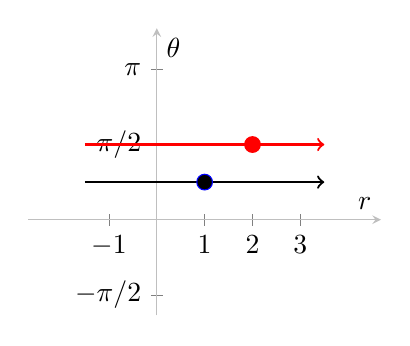
\begin{tikzpicture}
		\begin{axis}[
		xmin=-2,xmax=4,
		ymin=-2,ymax=4,
		ytick={-1.57,1.57,3.14},
		xtick={-1,1,2,3},
		yticklabels={$-\pi/2$,$\pi/2$, $\pi$},
		axis lines=middle,
		axis line style=lightgray,
		width=0.5\textwidth,
		xlabel={$r$},
		ylabel={$\theta$},
		axis equal
		] 
		
		\addplot[red,thick,->] expression[domain=-1.5:3.5,samples=2]{1.57};
		\node[color=red,draw=red,circle,fill,inner sep=2pt] at (axis cs:2,1.57) {}; 
		
		\addplot[black,thick,->] expression[domain=-1.5:3.5,samples=2]{1.57/2};
		\node[color=black,draw=blue,circle,fill,inner sep=2pt] at (axis cs:1,1.57/2) {}; 
		
		\end{axis}
		\end{tikzpicture}\hspace{1cm}
		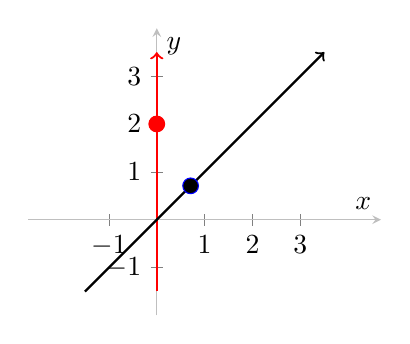
\begin{tikzpicture}
		\begin{axis}[
		xmin=-2,xmax=4,
		ymin=-2,ymax=4,
		ytick={-1,1,2,3},
		xtick={-1,1,2,3},
		axis lines=middle,
		axis line style=lightgray,
		width=0.5\textwidth,
		xlabel={$x$},
		ylabel={$y$},
		axis equal
		] 
		
		\addplot +[mark=none,red,thick,->] coordinates {(0, -1.5) (0, 3.5)};
		\node[color=red,draw=red,circle,fill,inner sep=2pt] at (axis cs:0,2) {}; 
		
		\addplot[black,thick,->] expression[domain=-1.5:3.5,samples=2]{x};
		\node[color=black,draw=blue,circle,fill,inner sep=2pt] at (axis cs:0.707,0.707) {}; 
		\end{axis}
		\end{tikzpicture}
		
		\mbox{}
		
		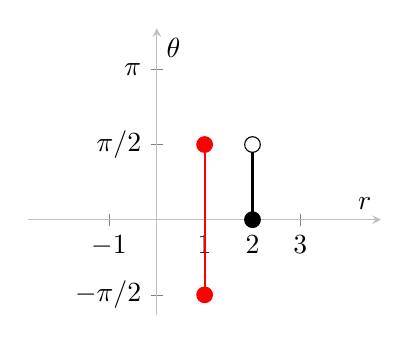
\begin{tikzpicture}
		\begin{axis}[
		xmin=-2,xmax=4,
		ymin=-2,ymax=4,
		ytick={-1.57,1.57,3.14},
		xtick={-1,1,2,3},
		yticklabels={$-\pi/2$,$\pi/2$, $\pi$},
		axis lines=middle,
		axis line style=lightgray,
		width=0.5\textwidth,
		xlabel={$r$},
		ylabel={$\theta$},
		axis equal
		] 
		
		\addplot +[mark=none,red,thick] coordinates {(1, -1.57) (1,1.57)};
		\node[color=red,draw=red,circle,fill,inner sep=2pt] at (axis cs:1,-1.57) {}; 
		\node[color=red,draw=red,circle,fill,inner sep=2pt] at (axis cs:1,1.57) {}; 
		
		\addplot +[mark=none,black,thick] coordinates {(2, 0) (2,1.57)};
		\node[color=black,draw=black,circle,fill,inner sep=2pt] at (axis cs:2,0) {}; 
		\node[color=white,draw=black,circle,fill,inner sep=2pt] at (axis cs:2,1.57) {}; 
		
		\end{axis}
		\end{tikzpicture}\hspace{1cm}
		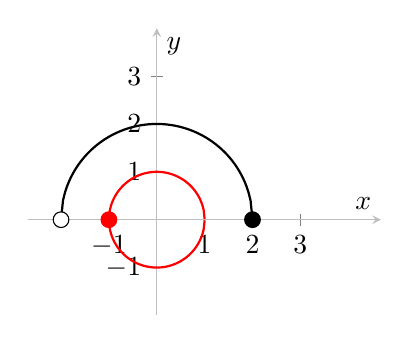
\begin{tikzpicture}
		\begin{axis}[
		xmin=-2,xmax=4,
		ymin=-2,ymax=4,
		ytick={-1,1,2,3},
		xtick={-1,1,2,3},
		axis lines=middle,
		axis line style=lightgray,
		width=0.5\textwidth,
		xlabel={$x$},
		ylabel={$y$},
		axis equal
		] 
		
		\addplot[red,thick] expression[domain=-1:1,samples=100]{sqrt(1-x^2)}; 
		\addplot[red,thick] expression[domain=-1:1,samples=100]{-sqrt(1-x^2)}; 
		\node[color=red,draw=red,circle,fill,inner sep=2pt] at (axis cs:-1,0) {}; 
		
		\addplot[black,thick] expression[domain=-2:2,samples=100]{sqrt(4-x^2)}; 
		\node[color=black,draw=black,circle,fill,inner sep=2pt] at (axis cs:2,0) {}; 
		\node[color=white,draw=black,circle,fill,inner sep=2pt] at (axis cs:-2,0) {}; 
		\end{axis}
		\end{tikzpicture}
	\end{center}
	\caption{The function $f(r, \theta) = (r\cos\theta, r\sin\theta)$ of \cref{polar-map} transforms the pictures on the right to the pictures on the left.}  \label{polar-map-picture}
\end{figure}

We compute partial derivatives. 
\[ \frac{\partial f_1}{\partial r} = \cos \theta \quad \frac{\partial f_2}{\partial r} = \sin \theta \quad \frac{\partial f_1}{\partial \theta} = -r\sin \theta \quad \frac{\partial f_2}{\partial \theta} = r\cos \theta.  \]
Thus
\[ f'(r, \theta) = \begin{bmatrix} \cos \theta & -r \sin \theta \\ \sin \theta & r \cos \theta \end{bmatrix}. \]
Since this is a square matrix, $df_{(r, \theta)}$ has non-maximal rank if and only if its determinant vanishes. But
\[ \det f'(r, \theta) = r\cos^2 \theta + r\sin^2 \theta = r, \]
so the critical locus\index{critical point!critical locus} (ie, the set of all critical points) of $f$ is the vertical line $r = 0$, and $f$ is \'etale away from this line. 
\end{example}

\begin{exercise}[Fold] \label{fold}
	Let $f : \R^2 \to \R^2$ be the function given by $f(x, y) = (x, y^2)$. 
	\begin{enumerate}[(a)]
		\item Draw pictures of $f$ (like the pictures in \cref{polar-map} above) until you can see why this function is called a ``fold.''
		\item What is the critical locus of $f$? 
	\end{enumerate}
\end{exercise}

\begin{exercise}[Parametrization of a cusp] \label{cusp}
	Consider the function $f : \R \to \R^2$ defined by
	\[ f(t) = (t^2, t^3). \]
	See \cref{cusp-graph} for a picture of the image of $f$. The ``pointy'' part at the origin is sometimes called a cusp\index{cusp}.
	\begin{figure}
			\begin{center}
			\begin{tikzpicture}
			\begin{axis}[
			xmin=-0.5,xmax=2,
			ymin=-2,ymax=2,
			ytick={0},
			xtick={0},
			xticklabels={},
			yticklabels={},
			axis lines=middle,
			axis line style=lightgray,
			width=0.75\textwidth
			]
			\addplot[black,style=thick,->] expression[domain=0:1.5,samples=50]{ sqrt(x^3) };
			\addplot[black,style=thick,-] expression[domain=0:1.5,samples=50]{ -sqrt(x^3) }; 
			\node[color=black,draw=black,circle,fill,inner sep=2pt] at (axis cs:0,0) {}; 
			
			\end{axis}
			\end{tikzpicture}
		\end{center}
	\caption{The image of the function $f(t) = (t^2, t^3)$. The origin is $f(0)$.}  \label{cusp-graph}
	\end{figure}
	Calculate $f'(t)$ for all $t \in \R$. Show that 0 is a critical point of $f$, and that $f$ is immersive away from 0.
\end{exercise}


\begin{exercise}[Parametrization of a node] \label{node}
	Consider the function $f : \R \to \R^2$ defined by
	\[ f(t) = (t^2-1, t^3-t). \]
	See \cref{node-graph} for a picture of the image of $f$. The self-intersecting part at the origin is called a node\index{node}. 
	\begin{figure}
		\begin{center}
			\begin{tikzpicture}
			\begin{axis}[
			xmin=-1.5,xmax=1,
			ymin=-1.5,ymax=1.5,
			ytick={0},
			xtick={},
			xticklabels={},
			yticklabels={},
			axis lines=middle,
			axis line style=lightgray,
			width=0.75\textwidth
			]
			\addplot[black,style=thick,->] expression[domain=-1:0.9,samples=500]{ sqrt(x^2*(x+1)) };
			\addplot[black,style=thick,-] expression[domain=-1:0.9,samples=500]{ - sqrt(x^2*(x+1)) }; 
			\node[label={$f(\pm1)$},color=black,draw=black,circle,fill,inner sep=2pt] at (axis cs:0,0) {}; 
			\node[label={120:$f(0)$},color=black,draw=black,circle,fill,inner sep=2pt] at (axis cs:-1,0) {}; 
			
			\end{axis}
			\end{tikzpicture}
		\end{center}
		\caption{The image of the function $f(t) = (t^2-1, t^3-t)$. We have $f(0) = (-1,0)$ and $f(\pm 1) = (0,0)$.}  \label{node-graph}
	\end{figure}
	Calculate $f'(t)$ for all $t \in \R$, and show that $f$ is immersive everywhere.
\end{exercise}

\begin{exercise}
	Show that an interior point $a \in S$ is a critical point\index{critical point} of $f : S \to \R$ if and only if $\partial_i f(a) = 0$ for all $i$. 
\end{exercise}

\begin{exercise} \label{sphere-fibration}
	Let $f : \R^3 \to \R$ be the function
	\[ f(x,y,z) = x^2 + y^2 + z^2 \]
	Calculate $f'(a)$ for all $a \in \R^3$, and find all critical points of $f$. Also, describe the level sets of $f$. In other words, for fixed $r \in \R$, describe the set of all $a \in \R^3$ such that $f(a) = r$. 
\end{exercise}

\begin{exercise}
	Find the critical points of the function $f : \R^3 \to \R^2$ given by \[ f(x,y,z) = (xy, z). \]
\end{exercise}

\begin{exercise}
	Find the critical points of the function $f : \R^3 \to \R^2$ given by \[ f(x,y,z) = (x+y^2, y+z^2). \]
\end{exercise}

\section{Differentiable functions}

We saw in \cref{differentiable-at-a-point-but-not-in-any-neighborhood} that a function that is differentiable at a point need not be differentiable at nearby points. Functions which are differentiable throughout an open set have some nice properties, which we discuss in this section. Throughout this section, $U$ denotes an open subset of $\R^m$. 

\begin{definition} \index{differentiable} \index{derivative}
	A function $f : U \to \R^n$ is \emph{differentiable} if it is differentiable at every $a \in U$. The \emph{differential} or the \emph{total derivative} of $f$, denoted $df$, is the function $U \to \mathscr{L}(\R^m, \R^n)$ given by $a \mapsto df_a$, where $\mathscr{L}(\R^m, \R^n)$ denotes the set of all linear maps $\R^m \to \R^n$.  
\end{definition}

\begin{definition}
	If $f : U \to \R$ and $h \in \R^m$ is a vector such that $\partial_h f(a)$ exists for all $a \in U$, then the \emph{directional derivative} of $f$ with respect to $h$ is the function $\partial_h f$ given by $a \mapsto \partial_h f(a)$. When $h = e_i$ is one of the standard basis vectors, this function is called the \emph{$i$th partial derivative} of $f$ and is denoted $\partial_i f$. If we're using the variable $x_i$ to denote the $i$th component of the input of $f$, then $\partial_i f$ is sometimes also denoted by one of the following. 
	\[ f_{x_i} \quad \frac{\partial f}{\partial x_i} \]
\end{definition}

\subsection{Convex subsets}

Recall that, in the single variable situation of \cref{single-differentiable}, a key role was played by functions defined on intervals. In the multivariable situation, a similar role is played by functions defined on ``convex'' subsets. These are subsets $S \subseteq \R^m$ such that any two points in $S$ can be joined by a straight line segment that never leaves $S$. 

\begin{definition} \label{straight-line-path}
	If $a, b \in \R^m$, the \emph{straight line path} from $a$ to $b$ is the function
	\[ \gamma(t) = (1-t)a + tb. \]
	Observe that $\gamma(0) = a$ and $\gamma(1) = b$. 
\end{definition}

\begin{exercise} \label{straight-line-path-differentiable}
	Show that, for any $a, b \in \R^m$, the straight line path from $a$ to $b$ is differentiable. 
\end{exercise}

\begin{definition} \label{convex}
	A subset $S$ of $\R^m$ is said to be \emph{convex} if, whenever $a, b \in S$ and $\gamma$ is the straight line path from $a$ to $b$, then $\gamma(t) \in S$ for all $t \in [0,1]$. 
\end{definition}

\begin{exercise}
	Determine whether or not
	\[ S = \{ (x, y) \in \R^2 : x \geq 0 \text{ or } y \neq 0 \} \]
	is a convex subset of $\R^2$. Justify your answer. 
\end{exercise}

\begin{exercise}
	Let $I$ be an interval. Suppose $f : I \to \R$ is concave down and $f \geq 0$. Show that
	\[ S = \{ (x, y) \in \R^2 : x \in I \text{ and } 0 \leq y \leq f(x) \} \]
	is a convex subset of $\R^2$. 
\end{exercise}

\subsection{Vanishing derivatives}

Here is a multivariable generalization of \cref{constant-iff-derivative-zero-single}. We will use the single variable version to prove this multivariable version. 

\begin{proposition} \label{constant-iff-derivative-zero}
	Suppose $U$ is convex and $f : U \to \R^n$ is a differentiable function. Then $df = 0$ if and only if $f$ is constant\index{constant function}.  
\end{proposition}

\begin{proof}
	Taking $w = 0$ in \cref{derivative-of-line} shows that, if $f$ is constant, then $df = 0$. For the converse, we can assume without loss of generality that $n = 1$ (cf. \cref{constant-iff-derivative-zero-details}). We want to show that, for any $a,  b \in U$, we have $f(a) = f(b)$. Let $\gamma$ be the straight line path from $a$ to $b$. Convexity of $U$ tells us that $\gamma(t) \in U$ for all $t \in [0,1]$. Also, $\gamma$ is differentiable by \cref{straight-line-path-differentiable}. Thus $f \circ \gamma$ is a differentiable function $[0,1] \to \R$ and 
	\[ (f \circ \gamma)'(t) = f'(\gamma(t)) \gamma'(t) = 0 \]
	where we used the (matrix version of the) chain rule \ref{chain-rule} at the second step, and the fact that $df = 0$ for the final step. Thus it follows from \cref{constant-iff-derivative-zero-single} that $f \circ \gamma$ is constant, which means that
	\[ f(a) = f(\gamma(0)) = f(\gamma(1)) = f(b). \qedhere \]
\end{proof}

\begin{exercise} \label{constant-iff-derivative-zero-details}
	 Explain why proving that $df = 0$ implies that $f$ is constant for $n = 1$ implies the same fact for general $n$. 
\end{exercise}

In fact, it's not necessary that the domain be convex in order for the conclusion of \cref{constant-iff-derivative-zero} to be true. Before getting to the general statement, here is a useful intuition-building exercise. 

\begin{exercise}
	Let $U$ denote $\R^2$ minus the non-negative $x$-axis. In other words,
	\[ U = \R^2 \setminus \{ (x, 0) \in \R^2 : x \geq 0 \}. \]
	\begin{enumerate}[(a)]
		\item Show that $U$ is not convex. 
		\item Suppose $f : U \to \R$ is a differentiable function such that $df = 0$. Show that $f$ is constant.
	\end{enumerate} 
	\begin{hint}
		Any pair of points in $U$ \emph{can} be joined by \emph{two} straight line paths...
	\end{hint}
\end{exercise}

\begin{exercise} \label{constant-iff-derivative-zero-connected}
	Let $U$ be a connected\footnotemark\ open subset of $\R^m$.
	\begin{enumerate}[(a)]
		\item Show that, for any $a, b \in U$, there exists a finite sequence of points \[ a = a_0, a_1, \dotsc, a_k = b \] such that the image of the straight line path between $a_i$ and $a_{i+1}$ is entirely contained in $U$ for all $i$. 
		
		\begin{hint}
			For $a \in U$, consider the set $S$ of all points $a' \in U$ such that there exists a finite sequence of points $a = a_0, a_1, \dotsc, a_k = a'$ such that the image of the straight line path connecting $a_i$ to $a_{i+1}$ is entirely contained in $U$ for all $i$. Show that $S$ is open, and also that the complement of $S$ is open. Since $U$ is connected and $S$ is nonempty, it must be that the complement of $S$ is empty.  
		\end{hint}
		
		\item If $f : U \to \R^n$ is differentiable, show that $df = 0$ if and only if $f$ is constant. 
	\end{enumerate}
\end{exercise}

\footnotetext{Recall that a metric space $X$ is \emph{connected}\index{connected} if it cannot be written as the union of two disjoint open subsets.}

\subsection{Bounded derivatives}

Here is a multivariable version of \cref{bounded-derivative}. Again, we will actually use the single variable version to prove the multivariable version. 

\begin{proposition} \label{bounded-derivative-multi}
	Suppose $U$ is convex and $f : U \to \R^n$ is a differentiable function. Suppose further that there exists a constant $M$ such that $\|df_x\| \leq M$ for all $x \in U$. Then
	\[ |f(b) - f(a)| \leq M |b-a| \]
	for all $a, b \in U$. 
\end{proposition}

\begin{proof}
	Suppose first that $n = 1$. If $a = b$, there is nothing to do, so we can assume that $a \neq b$. Let \[ h = \frac{b-a}{|b-a|}, \]
	ie, $h$ is the vector pointing from $a$ towards $b$ normalized to unit length. Consider the function $\xi(t) = a + th$ as in \cref{directional-to-single}. Then
	\[ (f \circ \xi)'(t) = \partial_h f(a + th) = df_{a + th}(h)  \]
	by \cref{jacobian-matrix}, which means that 
	\[ |(f \circ \xi)'(t)| = |df_{a + th}(h)| \leq \|df_{a + th}\| |h| \leq M|h| = M, \]
	where we used the fact that $h$ has unit length for the final step. Notice that $\xi(0) = a$ and $\xi(|b-a|) =  b$, so by applying \cref{bounded-derivative} to $f \circ \xi$, we see that 
	\[ |f(b) - f(a)| \leq M||b-a| - 0| = M|b-a|.  \]
	This proves the statement for $n = 1$.
	
	We'll prove the statement for general $n$ only for the max norm and the max operator norm. The proof for the euclidean norm is trickier: see \cite[theorem 9.19]{rudin}. Note that $df_{j,a} = \pi_j \circ df_a$ and $\|\pi_j\|_\infty = 1$ so \[ \|df_{j,a}\|_\infty \leq \|\pi_j\|_\infty \|df_a\|_\infty \leq M \]
	by \cref{operator-norm-submultiplicative}. Applying \cref{bounded-derivative-multi} to the component functions $f_j$, we find that 
	\[ |f_j(b) - f_j(a)| \leq M|b-a| \]
	for all $a, b \in B$ and all $j = 1, \dotsc, n$. Taking the maximum over all $j$ proves the result. 
\end{proof}

\begin{exercise}
	\begin{enumerate}[(a)]
		\item The statement of the \cref{bounded-derivative-multi} requires that the domain of $f$ is convex. Where in the proof is this used?
		\item Prove that $\|\pi_j\|_2 = \|\pi_j\|_\infty = 1$. 
		\item If you haven't already done it, do \cref{operator-norm-submultiplicative}. 
	\end{enumerate} 
\end{exercise}

\subsection{Inverse function theorem}

The inverse function theorem is an extremely important foundational result. It comes up frequently in real analysis and differential geometry, and has inspired significant developments in algebraic geometry and number theory. 

\begin{definition}
	A differentiable function $f : U \to \R^n$ is \emph{\'etale} if it is \'etale at every $a \in U$ (ie, if $df_a$ is an isomorphism for every $a \in U$). 
\end{definition}

\begin{theorem}[Inverse function theorem] \label{inverse-function-theorem}
	Suppose $f : U \to \R^n$ is \'etale. Then $f$ is open. Moreover, for every $a \in U$, there exists an open neighborhood $V$ of $a$ such that $f|_V$ is injective, the inverse function $(f|_V)^{-1}$ is differentiable, and
	\[ d((f|_V)^{-1})_y = (df_{(f|_V)^{-1}(y)})^{-1} \]
	for all $y  \in f(V)$. 
\end{theorem}

The proof will require an extremely lengthy discussion. For the time being, let us content ourselves with thinking about the statement of the theorem. 

First off, let us compare the statement against the single variable version of \cref{inverse-function-theorem-single}. If $I$ is an open interval in $\R$, then $f : I \to \R$ is \'etale if and only if it is differentiable and $f'(x)$ never vanishes, so the hypotheses of the theorem above and the single variable version match up exactly. The multivariable version above asserts that $f$ must be open and ``locally injective.'' On the other hand, the single variable version asserts that $f$ is strictly monotone; and we've seen that strict monotonicity implies that $f$ is open and injective (cf. \cref{strictly-monotone-iff-injective,strictly-monotone-implies-open}). The assertion on the differentiability of the inverse and the formula for the derivative of the inverse match up exactly.  

Thus, the single variable version is a stronger statement (when it applies) because it guarantees full injectivity everywhere on the domain, whereas the multivariable version above only guarantees ``local injectivity'' near every point of the domain. This is the only difference between the two statements, and here is an example to show that we cannot expect full injectivity in the multivariable setting.  

\begin{exercise} \label{locally-injective-not-injective}
	Consider the function $f : \R^2 \to \R^2$ given by 
	\[ f(x,y) = (e^x \cos y, e^x \sin y). \]
	\begin{enumerate}[(a)]
		\item Compute $df$ and verify that $f$ is \'etale. 
		\item Show that $f$ is \emph{not} injective. In fact, for any point $(a,b)$ in the range, show that there exist infinitely many points in the domain which map to $(a,b)$.
		\item Find an open neighborhood $V$ of the origin such that $f|_V$ is injective. 
	\end{enumerate}
\end{exercise}

Another important observation about the statement is the following. The inverse function theorem asserts that being \'etale is \emph{sufficient} to guarantee the existence of (local) inverses. It is \emph{not} a necessary condition for the existence of inverses, but it \emph{is} a necessary condition for the existence of \emph{differentiable} inverses, as shown by the following exercise. 

\begin{exercise}
	\begin{enumerate}[(a)]
		\item Give an example of a differentiable and injective function $f : \R \to \R$ which is not \'etale. What is the inverse of your function $f$? Is the inverse differentiable? 
		\item Suppose $U$ is an open subset of $\R^n$ such that $f : U \to \R^n$ is differentiable and injective and that $f(U)$ is open. Show that, if $f^{-1} : f(U) \to \R^n$ is differentiable, then $f$ is \'etale.  
	\end{enumerate}
\end{exercise}

The importance of the inverse function theorem derives from the fact that it lets us use linear algebra (which is easy) to make assertions about solutions of nonlinear equations (which are very difficult, in general). Here is an example to illustrate this point. 

\begin{example}
	Consider the following nonlinear system of equations. 
	\[ \begin{aligned} x + x^2y &= a \\ y - xy^2 + 3x^2 &= b \end{aligned} \]
	When $a = b = 0$, this system has a solution given by $x = y = 0$. That much is clear. What if $a$ and $b$ are not both zero? Does this system have any solutions? Are the solutions unique at all? None of this is very obvious on the face of it. I at least do not see any clear way to solve for $x$ and $y$ in terms of $a$ and $b$.  
	
	Let $f : \R^2 \to \R^2$ be the function given by $f(x,y) = (x+x^2y, y - xy^2 + 3x^2)$. Then 
	\[ \det f'(x,y) = \det \begin{bmatrix} 1 + 2xy & x^2 \\ 6x -y^2 & 1 - 2xy \end{bmatrix} = 1 - 6x^3 - 3x^2y^2. \]
	This is a continuous function of $(x,y)$ and it is nonzero when $(x,y) = 0$, so there exists an open neighborhood $U$ of $0$ such that $\det f'(x,y) \neq 0$ for all $(x,y) \in U$. In other words, $f|_U$ is \'etale. By the inverse function theorem \ref{inverse-function-theorem}, we can replace $U$ with a smaller open neighborhood of 0 in order to guarantee that $f|_U$ is injective and open. Then $f(U)$ is an open neighborhood of $f(0) = 0$, and for every $(a,b) \in f(U)$, there exists a unique $(x,y) \in \R^2$ such that $f(x,y) = (a,b)$. 
	
	We have just proved that, for every $(a,b)$ in $f(U)$, the system has a unique solution given by $(x,y) \in U$. In other words, if we perturb $a$ and $b$ just a little bit away from 0, our system will have a unique solution close to 0. Thanks to the inverse function theorem \ref{inverse-function-theorem}, proving this boiled down to a simple linear algebra calculation!
\end{example}

Here are some more exercises and examples that may help clarify the statement of the inverse function theorem. 

\begin{exercise}
	Recall the function $f(x) = x + 2x^2 \sin(1/x)$ that we saw in \cref{positive-not-monotone}. As we've seen, $f'(0) = 1$ but $f$ is not monotone (hence not injective, by \cref{strictly-monotone-iff-injective}) on any open neighborhood of $0$. Explain why this does not violate the inverse function theorem. In other words, show that $f$ is not \'etale on any open neighborhood of 0.
\end{exercise}

\begin{exercise}
	Let $U = \{(x,y) \in \R^2 : x > 0\}$ and let $f : U \to \R^2$ be the function \[ f(x,y) = (xe^{-y}, xe^y). \]
	\begin{enumerate}[(a)]
		\item Show that $f$ is \'etale. 
		\item Show that $f$ is injective. What is $f(U)$?
		\item Calculate $(f^{-1})'(1,1)$. 
	\end{enumerate}
\end{exercise}

\subsection{Proof of the inverse function theorem \starred}

This section is devoted to the proof of the inverse function theorem \ref{inverse-function-theorem}. It's a long and arduous proof.

\subsubsection*{Differentiability of the local inverse}

As it turns out, once a local inverse has been constructed, proving that it is differentiable is not terribly difficult. The proof of this part is similar in spirit to the single variable version (cf. the proof of \cref{inverse-function-theorem-single}).

\begin{proposition} \label{inverse-differentiable}
	Suppose $f : U \to \R^n$ is differentiable, open, and injective. Then $f^{-1}$ is differentiable and \[ d(f^{-1})_y = (df_{f^{-1}(y)})^{-1} \] for all $y \in f(U)$. 
\end{proposition}

\begin{proof}
	Fix $x \in U$ and $y = f(x)$. Let
	\[ s(k) = f^{-1}(y + k) - f^{-1}(k) - df_x^{-1}(k). \]
	We want to show that $|s(k)| = o(|k|)$ as $k \to 0$. In fact, since $df_x$ is an invertible linear map, it is sufficient to show that $|df_x(s(k))| = o(|k|)$ (cf. \cref{chain-rule-details} part  (\ref{linear-of-small-is-small})). 
	
	Define \[ h(k) = f^{-1}(y + k) - f^{-1}(y). \]
	Since $f$ is injective, we see that $h(k) = 0$ if and only if $k = 0$. Moreover, $f^{-1}$ is continuous since $f$ is open, which implies that $h$ is also continuous. Now by rewriting $s$ in terms of $h$, we have the following. 
	\[ \begin{aligned} 
	s(k) &= h(k) - df_x^{-1}(k) \\
	df_x(s(k)) &= df_x(h(k)) - k \\
	&= df_x(h(k)) - y + k + y \\
	&= df_x(h(k)) - f(x+h(k)) + f(x). \end{aligned} \]
	In other words, if we consider the ``error in approximation'' function
	\[ r(h) = f(x+h) - f(x) - df_x(h), \]
	then
	\[ df_x(s(k)) = -r(h(k)) \]
	for all $k$. This means that, for all $k \neq 0$, we have
	\[ \frac{|df_x(s(k))|}{|k|} = \frac{|r(h(k))|}{|k|} = \frac{|r(h(k))|}{|h(k)|} \cdot \frac{|h(k)|}{|k|} \]
	where we have used the fact that $h(k) \neq 0$ since $k \neq 0$. Now, since $|r(h)| = o(|h|)$ as $h \to 0$ and since the function $h$ is continuous at $k = 0$, we have that 
	\[ \lim_{k \to 0} \frac{|r(h(k))|}{|h(k)|} = 0. \]
	Thus it is sufficient to show that there exists a constant $M$ such that $|h(k)| \leq M|k|$ for all sufficiently small values of $k$.
	
	Since $|r(h)| = o(|h|)$ as $h \to 0$, there exists $\delta > 0$ such that $|r(h)| \leq |h|$ for all $|h| < \delta$. Then we have 
	\[ \begin{aligned} |h| &\geq |r(h)| = |f(x+h) - f(x) - df_x(h)| \\ &\geq |df_x(h)| - |f(x+h) - f(a)| \\
	&\geq \frac{|h|}{\|df_x^{-1}\|} - |f(x+h)-f(x)| \end{aligned} \]
	where we have used \cref{operator-norm-inverse} for the final step. After rearranging, this becomes
	\[ |h| \leq \left(\frac{1}{\|df_x^{-1}\|} - 1\right)^{-1} |f(x+h) - f(x)|. \] 
	Set
	\[ M = \left(\frac{1}{\|df_x^{-1}\|} - 1\right)^{-1}. \]
	Now if $h = h(k)$, we have $f(x+h(k)) - f(x) = k$, so the last inequality displayed above reads
	\[ |h(k)| \leq M |f(x+h(k)) - f(x)| = M|k|. \qedhere \]
\end{proof}

\subsubsection*{Reductions}

For the remainder of this proof, $f : U \to \R^n$ will denote an \'etale map. In particular, this means that $m = n$, ie, that $U$ is an open subset of $\R^n$. We'll closely follow  \href{https://terrytao.wordpress.com/2011/09/12/the-inverse-function-theorem-for-everywhere-differentiable-maps/#more-5298}{Terry Tao's exposition} of Saint Raymond's proof \cite{saint-raymond}. 

Let's begin by making a couple of helpful definitions. 

\begin{definition}
	For any point $a \in U$, we make the following definitions. 
	\begin{itemize}
		\item We say that $f$ is \emph{locally injective at $a$} if there exists an open neighborhood $V$ of $a$ such that $f|_V$ is injective. 
		\item We say that $f$ is \emph{locally surjective at $a$} if $f(a)$ is an interior point of $f(V)$ for every open neighborhood $V$ of $a$. 
	\end{itemize}
\end{definition}

\begin{exercise} \label{open-iff-locally-surjective}
	Show that $f$ is open if and only if $f$ is locally surjective at every $a \in U$. 
\end{exercise}

\begin{solution}{\cref{open-iff-locally-surjective}}
	This is just unwinding definitions. Suppose $f$ is open. Fix a point $a \in U$ and let $V$ be an open neighborhood of $a$ in $U$. Since $f$ is open, $f(V)$ is open, so $f(a)$ must be an interior point of $f(V)$. Conversely, suppose $f$ is locally surjective at every point in $U$. Let $V$ be an open subset of $U$. If $b \in f(V)$, there is an $a \in V$ such that $f(a) = b$. But $f$ is locally surjective at $a$, so $f(a) = b$ is an interior point of $f(V)$. Thus every $b \in f(V)$ is an interior point of $f(V)$, so $f(V)$ is open. 
\end{solution}

In other words, to prove the inverse function theorem, we want to show that $f$ is locally injective and locally surjective at every point $a \in U$. We can replace $f$ with the function $x \mapsto f(x+a)$ in order to assume that $a = 0$. Then, we can replace $f$ with the function $x \mapsto f(x) - f(0)$ in order to assume that $f(0) = 0$. Finally, since $df_0$ is invertible, we can replace $f$ with $df_0^{-1} \circ f$ in order to assume that $df_0 = \id$. 

\begin{exercise} \label{wlog-inverse-function-theorem}
	Check that you understand the ``we can assume''s in the previous paragraph. More precisely, suppose $a \in U$, $\ell : \R^n \to \R^n$ is a linear map, $\alpha_0 \in \R^n$, and $\alpha : \R^n \to \R^n$ is the function \[ \alpha(x) = \ell(x) + \alpha_0. \]
	Prove the following facts. 
	\begin{enumerate}[(a)]
		\item Show that $\alpha$ is bijective, and calculate $d\alpha$ and $d\alpha^{-1}$. 
		\item Let $\tilde{f} = \alpha \circ f$. 
		\begin{itemize}
			\item Show that $f$ is \'etale if and only if $\tilde{f}$ is \'etale. 
			\item Show that $f$ is locally injective at $a$ if and only if $\tilde{f}$ is locally injective at $a$. 
			\item Show that $f$ is locally surjective at $a$ if and only if $\tilde{f}$ is locally surjective at $a$.
		\end{itemize}  
		\item Let $\tilde{f} : \alpha^{-1}(U) \to \R^n$ be the composite $\tilde{f} = f \circ \alpha$. 
			\begin{itemize}
				\item Show that $f$ is \'etale if and only if $\tilde{f}$ is \'etale. 
				\item Show that $f$ is locally injective at $a$ if and only if $\tilde{f}$ is locally injective at $\alpha^{-1}(a)$. 
				\item Show that $f$ is locally surjective at $a$ if and only if $\tilde{f}$ is locally surjective at $\alpha^{-1}(a)$.
			\end{itemize} 
		\item Figure out what $\ell$ and $\alpha_0$ are for each of the ``we can assume''s of the previous paragraph. 
	\end{enumerate}
\end{exercise}

In other words, we want to show that, if $f$ is an \'etale map such that $f(0) = 0$ and $df_0 = \id$, then $f$ is locally injective and locally surjective at 0. Local surjectivity is easier; local injectivity is very, very difficult. 

\subsubsection*{Local surjectivity}

Since $f(0) = 0$ and $df_0 = \id$, we have $|f(h) - h| = o(|h|)$ as $h \to 0$ by the definition of the derivative, so there exists $\delta > 0$ such that 
\begin{equation} \label{inverse-function-theorem-eqn1} |f(h)-h| \leq |h|/2 \end{equation}
for all $|h| < \delta$. Replacing $f$ with the function $x \mapsto f(x/\delta)$, we can assume without loss of generality that $\delta = 1$ (cf. \cref{wlog-inverse-function-theorem}). We now claim that for all $0 < r < 1$, we have
\begin{equation} \label{inverse-function-theorem-locally-surjective} B(0,r/3) \subseteq f(B(0,r)). \end{equation}
Suppose $b \in B(0, r/3)$. Let $\nu : \R^m \to \R$ be the differentiable function given by $\nu(x) = x_1^2 + \dotsb x_n^2$ and then consider the function $\sigma : \overline{B}(0,r) \to \R$ given by \[ \sigma(x) = \nu(f(x)-b). \]
Since $\overline{B}(0,r)$ is compact, this function must attain its minimum at a point $a \in \overline{B}(0,r)$. We will show that $a \in B(0,r)$ and that $f(a) = b$, thus proving \cref{inverse-function-theorem-locally-surjective}. 

First of all, we must have $a \in B(0,r)$. Suppose for a contradiction that $|a| = r$. Then by \cref{inverse-function-theorem-eqn1} we would have
\[ r/2 \geq |f(a)-a| \geq |a| - |f(a)| = r - |f(a)| > 2r/3, \]
where we've used the reverse triangle inequality for the second step. This is evidently contradiction, since $r/2 < 2r/3$. In other words, we have proved that $a$ is an interior point of the domain of $\sigma$. 

Now we prove that $f(a) = b$. The chain rule \ref{chain-rule} tells us that 
\[ d\sigma_{a} = d\nu_{f(a)-b} \circ df_{a}. \]
Since the interior point $a$ is the absolute minimum of $\sigma$, the interior extremum theorem \ref{interior-extremum-directional} and \cref{jacobian-matrix} tells us that $d\sigma_a = 0$, which means that $df_a(\R^n) \subseteq \ker(d\nu_{f(a)-b})$. Since $df_a$ is invertible, this means that $d\nu_{f(a)-b} = 0$. But we have 
\[ \nu'(x) = \begin{bmatrix} 2x_1 & 2x_2 & \dotsb & 2x_n \end{bmatrix} \]
so $d\nu_{f(a) - b} = 0$ if and only if $f(a) - b = 0$. We have now proved \cref{inverse-function-theorem-locally-surjective}. 

Notice that \cref{inverse-function-theorem-locally-surjective} implies that $f$ is locally surjective at 0. Indeed, any open neighborhood $V$ of 0 contains an open ball of the form $B(0,r)$ for $0 < r < 1$, and then \[ f(V) \supseteq f(B(0,r)) \supseteq B(0,r/3), \] so $f(0) = 0$ is an interior point of $f(V)$. 

\subsubsection*{Local injectivity under assumptions}

Proving local injectivity in general is very challenging, but is a bit easier if we add some hypotheses to the statement of the theorem. In this section, we look at some of these arguments under additional assumptions. 

\mbox{}

\noindent \textit{Assuming $n = 1$.} As we've already noted, we've already proved not just local injectivity but full injectivity when $n = 1$ in \cref{inverse-function-theorem-single}. In any case, it's worth isolating the argument of injectivity and inspecting it closely. 

Suppose we have $a_1 < a_2$ such that $f(a_1) = f(a_2)$. We'll prove that this leads to a contradiction using two different but very similar arguments. The first argument is very quick. The mean value theorem guarantees that there exists $\xi$ between $a_1$ and $a_2$ such that $f'(\xi) = 0$, which contradicts our assumption that $f$ is \'etale. 

The second argument avoids using the mean value theorem basically by proving the mean value theorem for this particular situation. The idea is to set $b := f(a_1) = f(a_2)$ and consider the function \[ \sigma(x) = (f(x)-b)^2. \]
Since $\sigma$ is a continuous function on the compact interval $[a_1, a_2]$, the extreme value theorem guarantees that it attains its maximum at some point $\xi \in [a_1, a_2]$. Observe that $\sigma(a_1) = \sigma(a_2) = 0$ and $\sigma \geq 0$, so if $\sigma(\xi) = 0$, then $\sigma = 0$ constantly, so $f$ is constantly equal to $b$, which means the derivative vanishes on $(a_1, a_2)$ by \cref{constant-iff-derivative-zero}, contradicting our assumption that $f$ is \'etale. Thus $\sigma(\xi)$ must be an interior point of the interval $(a_1, a_2)$ and $\sigma(\xi) \neq 0$, ie, $f(\xi) \neq b$. Then the interior extremum theorem \ref{interior-extremum} plus the chain rule tells us that
\[ 0 = \sigma'(\xi) = 2(f(\xi) - b)f'(\xi).  \]
Since $f(\xi) \neq b$, this says that $f'(\xi) = 0$, which again contradicts our assumption that $f$ is \'etale. 

This second argument is useful because the proof in the general setting involves maximizing a multivariable function that's very similar to the single variable function $\sigma$ above. But before we get to the general proof, here is another proof under additional hypotheses. 

\mbox{}

\noindent \textit{Assuming continuous differentiability.} We haven't formally defined it yet, but $f$ is said to be ``continuously differentiable'' if all of the partial derivatives of the component functions $\partial_i f_j$ are continuous (cf. \cref{continuously-differentiable-definition}). The proof that $f$ is locally injective at 0 is a little easier if we assume that $f$ is continuously differentiable, but still a little tricky. The proof here is essentially the one from \cite[chapter 2]{spivak_calculus}. 

Since $df_0 = \id$, we know that $\partial_i f_j(0) = \delta_{i,j}$. Since $\partial_i f_j$ is continuous at 0, there exists $\delta > 0$ such that 
\[ |\partial_i f_j(0) - \partial_i f_j(x)| = |\delta_{i,j} - \partial_i f_j(x)| \leq \frac{1}{2n}. \]
Let $V = B(0,\delta)$. We will show that $f|_V$ is injective. 

Let $g(x) = x - f(x)$. It turns out that it is sufficient to prove that $\|dg_x\| \leq 1/2$ for all $x \in V$. Indeed, if we can prove this, then \cref{bounded-derivative-multi} would tell us that 
\[ |g(x_1) - g(x_2)| \leq \frac{1}{2} |x_1 - x_2| \]
for all $x_1, x_2 \in V$. But
\[ |g(x_1) - g(x_2)| = |(x_1 - f(x_1)) - (x_2 - f(x_2))| \geq |x_1 - x_2| - |f(x_1) - f(x_2)| \]
by the reverse triangle inequality. This leads to the following. 
\[ \begin{aligned} |x_1 - x_2| - |f(x_1) - f(x_2)| &\leq \frac{1}{2} |x_1 - x_2| \\
\frac{1}{2}|x_1 - x_2| &\leq |f(x_1) - f(x_2)| \\
|x_1 - x_2| &\leq 2|f(x_1) - f(x_2)| \end{aligned} \]
This shows that $f(x_1) = f(x_2)$ if and only if $x_1 = x_2$, or, in other words, that $f|_V$ is injective. 

We'll prove that $\|df_x\| \leq 1/2$ only for the max norm (and, correspondingly, the max operator norm). Observe that $\partial_i g_j(x) = \delta_{i,j} - \partial_i f_j(x)$, so we have 
\[ |g'(x)|_\infty = \max_{i,j} |\partial_i g_j(x)| \leq \frac{1}{2n} \]
for all $x \in V$. Using \cref{max-matrix-norm-and-max-operator-norm}, we see that $\|dg_x\|_\infty \leq 1/2$ for all $x \in V$. 

\begin{unimportantremark}
	It is also true that $\|dg_x\|_2 \leq 1/2$. To prove this, we would use the fact that $\|\ell\|_2 \leq \sqrt{mn}|A|_\infty$ when $A$ is the standard matrix representation of a linear map $\ell : \R^m \to  \R^n$ (cf. \cite[section 2.3.2]{golub}), instead of \cref{max-matrix-norm-and-max-operator-norm}. In any case, we didn't prove \cref{bounded-derivative-multi} for the eucldiean norm situation, so perhaps its better to stick with the max norm here anyway. 
\end{unimportantremark}

\subsubsection*{Local injectivity}
	
{\color{blue} Incomplete. I'll write this up eventually. The continuously differentiable case we proved above is really sufficient almost all of the time (and is all we'll use as we go forward), but if you're really curious about the general case, look at \href{https://terrytao.wordpress.com/2011/09/12/the-inverse-function-theorem-for-everywhere-differentiable-maps/#more-5298}{Terry Tao's blog post}.}
% TODO: Local injecticity for inverse function theorem

% TODO: Implicit function theorem

\section{\texorpdfstring{$C^k$}{Ck} hierarchy}

Throughout this section, $U$ denotes an open subset of $\R^m$.

\subsection{Continuous differentiability}

\subsubsection*{Continuity of partials}

The following theorem is the promised sort-of-converse to \cref{differentiable-implies-directionals}. Recall from \cref{partials-dont-imply-differentiable} above that the partial derivatives all existing everywhere is \emph{not} sufficient to guarantee differentiability. But, insisting that the partial derivatives all exist \emph{and are continuous} turns out to be enough to guarantee differentiability of $f$. The proof is harder than you might expect. 

\begin{theorem} \label{continuous-partials}
	Suppose $f : U \to \R$ is a function such that the $i$th partial derivative $\partial_i f : U \to \R$ exists for all $i = 1 , \dotsc m$. If $a \in U$ is a point such that $\partial_i f$ is continuous at $a$ for all $i$, then $f$ is differentiable at $a$. 
\end{theorem}

\begin{proof}[Proof]
	If $f$ is to be differentiable at $a$, we know from \cref{jacobian-matrix} what $df_a$ needs to be in terms of the partial derivatives; so let's turn this on its head by writing down the linear map defined by the partial derivatives, and then proving that that linear map is in fact $df_a$. 
	
	More precisely, we mean the following. Let $\ell$ be the linear map $\R^m \to \R$ such that \[ [\ell] = \begin{bmatrix}
	\partial_1f(a) & \dotsb & \partial_m f(a)
	\end{bmatrix}. \]
	In other words, $\ell : \R^m \to \R$ is the linear map given by
	\[ \ell(h_1, \dotsc, h_m) = h_1 \partial_1 f(a) + \dotsb + h_m \partial_m f(a). \]
	We will show that 
	\[ |f(a+h) - f(a) - \ell(h)| = o(|h|) \text{ as } h \to 0, \]
	which implies that $f$ is differentiable at $a$ and that $df_a = \ell$. In other words, we will show that, for any $\epsilon > 0$, there exists a $\delta > 0$ such that, for all $h \in \R^m$ with $|h| < \delta$, we have
	\begin{equation} \label{continuous-differentiability-desired} |f(a+h) - f(a) - \ell(h)| \leq |h|\epsilon. \end{equation}
	
	Let $\delta_0 > 0$ be small enough that $B(a, \delta_0) \subseteq U$. We will soon make it smaller to get inequality \eqref{continuous-differentiability-desired} to hold, but for the moment it is sufficient that $B(a, \delta_0) \subseteq U$. 
	Suppose $h = (h_1, \dotsc, h_m) \in \R^m$ with $|h| < \delta_0$. Then consider the following vectors in $\R^m$. 
	\[ \begin{aligned} 
	a_0 &= a \\
	a_1 &= a + (h_1, 0, 0 \dotsc, 0, 0) \\
	a_2 &= a + (h_1, h_2, 0, \dotsc, 0, 0) \\
	&\enspace \vdots \\
	a_{m-1} &= a + (h_1, h_2, h_3, \dotsc, h_{m-1}, 0) \\
	a_m &= a + (h_1, h_2, h_3, \dotsc, h_{m-1}, h_m) = a + h \end{aligned} \]
	The vectors $a_0, \dotsc, a_m$ define a sort of ``zigzag path'' from $a$ to $a + h$. See \cref{continuous-differentiability-picture}. Clearly $a_i \in B(a, \delta_0)$ for all $i = 1, \dotsc, m$. 
	\begin{figure}
		\begin{center}
			\begin{tikzpicture}
			\begin{axis}[
			xmin=-0.1,xmax=3,
			ymin=-0.1,ymax=3,
			ytick={0},
			xtick={0},
			xticklabels={0},
			yticklabels={0},
			axis lines=middle,
			axis line style=lightgray,
			axis equal,
			width=0.75\textwidth
			]
			\addplot[black,dotted,-] expression[name path=a,domain=0.5:2.5,samples=100]{2.5}; 
			\addplot[black,dotted,-] expression[name path=b,domain=0.5:2.5,samples=100]{0.5}; 
			\addplot[fill=gray, fill opacity=0.05
			]
			fill between[of=a and b,soft clip={domain=0.5:2.5}];
			\addplot +[mark=none,black,dotted] coordinates {(0.5, 0.5) (0.5, 2.5)};
			\addplot +[mark=none,black,dotted] coordinates {(2.5, 0.5) (2.5, 2.5)};
			
			
			\node[label={235:$a$},color=black,draw=black,circle,fill,inner sep=2pt] at (axis cs:1.5,1.5) {}; 
			\node[label={90:$a+h$},color=black,draw=black,circle,fill,inner sep=2pt] at (axis cs:2.2,1.9) {}; 
			\node[label={315:$a_1$},color=black,draw=black,circle,fill,inner sep=2pt] at (axis cs:2.2,1.5) {};
			
			\addplot[black,-] expression[domain=1.5:2.2,samples=2]{1.5};
			\addplot +[mark=none,black,solid] coordinates {(2.2, 1.5) (2.2, 1.9)};
			\end{axis}
			\end{tikzpicture}
		\end{center}
		\caption{A picture of $a, a_1$ and $a_2 = a + h$, as defined in the proof of \cref{continuous-partials}. Defining $\xi_1$ and $\xi_2$ using the mean value theorem as in the proof, the point $a + \xi_1e_1$ is somewhere along the horizontal line joining $a$ and $a+h_1$, and the point $a+h_1 + \xi_2e_2$ is somewhere on the vertical line joining $a+h_1$ and $a+h$.}  \label{continuous-differentiability-picture}
	\end{figure}
	
	Notice that 
	\[ f(a+h) - f(h) = \sum_{i = 1}^m \left( f(a_i) - f(a_{i-1}) \right). \]
	Let us fix $i$ temporarily. Notice that $a_i = a_{i-1} + h_i e_i$, so
	\[ f(a_i) - f(a_{i-1}) = f(a_{i-1}+h_ie_i) - f(a_{i-1}). \]
	Suppose $h_i \neq 0$. We can then apply the mean value theorem \ref{mean-value-theorem}\index{mean value theorem} to the single variable function \[ t \mapsto f(a_{i-1} + te_i) \] on the closed interval between $0$ and $h_i$. This function is well-defined and differentiable on this interval: its derivative at a value $t$ is $\partial_i f(a_{i-1} + te_i)$, by definition of partial derivatives. The mean value theorem \ref{mean-value-theorem}\index{mean value theorem} says that there exists $\xi_i$ between 0 and $h_i$ such that
	\[ \partial_i f(a_{i-1} + \xi_ie_i) = \frac{f(a_{i-1} + h_ie_i) - f(a_{i-1})}{h_i} = \frac{f(a_{i}) - f(a_{i-1})}{h_i}, \]
	or, in other words,
	\[ f(a_i) - f(a_{i-1}) = \xi_i \partial_i f(a_{i-1} + \xi_i e_i). \]
	If $h_i = 0$, we set $\xi_i = 0$ as well. 
	See \cref{continuous-differentiability-picture} again. Unfixing $i$, we find that
	\[ f(a+h) - f(a) = \sum_{i = 1}^m (f(a_i) - f(a_{i-1})) = \sum_{i = 1}^m \xi_i \partial_i f(a_{i-1} + \xi_i e_i). \]
	Thus
	\[ |f(a+h) - f(a)-\ell(h)| \leq \sum_{i = 1}^m |\xi_i| \cdot |\partial_i(a_{i-1}+\xi_ie_i) - \partial_if(a)|. \]
	Since $\partial_if$ is continuous at $a$, there exists $\delta_i > 0$ such that $|\partial_i(a+k) - \partial_i(a)| < \epsilon/m$ for all $|k| < \delta_i$. Let $\delta = \min\{\delta_0, \delta_1, \dotsc, \delta_m\}$. If $|h| < \delta$, then 
	\[ |\partial_i(a_{i-1} + \xi_ie_i) - \partial_i f(a)| < \epsilon/m, \]
	which means that
	\[ |f(a+h) - f(a)-\ell(h)| \leq \sum_{i = 1}^m \frac{|\xi_i| \epsilon}{m} = \frac{\epsilon}{m} \sum_{i = 1}^m |\xi_i| \leq |h| \epsilon , \]
	where we use the fact that $|\xi_i| \leq |h_i|$ for all $i$ for the final step. 
\end{proof}

\begin{unimportantremark}
	If you're using the euclidean norm, you'll have to apply \cref{max-euclidean} for the final step of the proof above. This is another example of why the max norm is often easier to deal with. 
\end{unimportantremark}

Here is another fact that can be proved using a similar argument involving zigzag paths where each segment is orthogonal to the coordinate axes. 

\begin{exercise}
	Suppose $U$ is a convex open subset of $\R^m$ and $f : \R^m \to \R$ is a (not necessarily differentiable) function for which there exists a constant $M > 0$ such that $|\partial_i f(x)| \leq M$ for all $i = 1, \dotsc, m$ and $x \in U$. Prove that $f$ is continuous. 
\end{exercise}

\subsubsection*{Continuous differentiability}

\begin{definition}[Continuously differentiable functions] \index{continuously differentiable} \label{continuously-differentiable-definition}
	We say that $f$ is \emph{continuously differentiable} if $\partial_i f_j : U \to \R$ is continuous for all $i = 1, \dotsc, m$ and $j = 1, \dotsc, n$. \Cref{continuous-partials} guarantees that such a function is, in particular, differentiable. 
\end{definition}

As we saw in the single variable case, continuously differentiable functions have lots of nice properties. For example, recall the calculation we did in \cref{polar-map} showing that the critical locus was a line inside $\R^2$, which is a closed subset. This fact is a special case of the following.

\begin{exercise} \label{critical-locus-closed}
	Suppose $f : U \to \R^n$ is continuously differentiable. Show that the ``critical locus'' of $f$ (ie, the set of all critical points of $f$) is a closed subset of $U$.
\end{exercise}

Here is a multivariable version of the differentiable-but-not-continuously-differentiable function from \cref{power-times-sine}. 

\begin{exercise}
	Let $f : \R^2 \to \R$ denote the following function.
	\[ f(x, y) = \begin{cases} x^2\sin(1/x) + y^2\sin(1/y) & \text{if } x, y \neq 0 \\
	x^2\sin(1/x) & \text{if } x \neq 0 \text{ and } y = 0 \\
	y^2\sin(1/y) & \text{if } x = 0 \text{ and } y \neq 0 \\
	0 & \text{if } x = y = 0 \end{cases} \]
	Show that $f$ is differentiable, but not continuously differentiable. 
\end{exercise}

\begin{exercise} \label{no-continously-differentiable-bijection}
	You might recall proving at some point in a previous class that $\R^2$ and $\R$ have the same cardinality: in other words, that there exists a bijection $f : \R^2 \to \R$. Show that any such bijection cannot be continuously differentiable. 
	
	\begin{hint}
		Suppose for a contradiction that $f : \R^2 \to \R$ is a continuously differentiable bijection.  Let $U$ be an open subset of $\R^2$ such that $\partial_1 f(x, y) \neq 0$ for all $(x,y) \in U$, and then consider the function $g : U \to \R^2$ given by $g(x, y) = (f(x, y), y)$. 
	\end{hint}
\end{exercise}

\begin{proposition} \label{c1-stable-inversion}
	Suppose $f : U \to \R^n$ is continuously differentiable, open, and injective. Then $f^{-1}$ is also continuously differentiable. 
\end{proposition} 

\begin{proof}
	We know from \cref{inverse-differentiable} that $f^{-1}$ is differentiable and that  
	\[ d(f^{-1})_y = (df_{f^{-1}(y)})^{-1} \]
	for all $y \in U$. Taking standard matrix representations, we get
	\[ [d(f^{-1})_y] = [(df_{f^{-1}(y)})^{-1}] = [df_{f^{-1}(y)}]^{-1}.  \]
	By \cref{jacobian-matrix}, the $(j,i)$-entry on the left hand side is $\partial_i (f^{-1})_j(y)$, so this equality says that $\partial_i (f^{-1})_j : f(U) \to \R$ is equal to the following composite. 
	\[ \begin{tikzcd} f(U) \ar{r}{f^{-1}} & U \ar{rr}{x \mapsto [df_x]} & & \GL_n \ar{rr}{A \mapsto A^{-1}} & & \GL_n \ar{rr}{(j,i)-\text{entry}} & & \R \end{tikzcd} \]
	Here $\GL_n$ denotes the set of invertible $n \times n$ matrices as in \cref{matrix-norm}. Each of the functions being composed here is continuous (cf. 
	\cref{differentiable-implies-continuous,matrix-inversion-homeomorphism}), so we conclude that $\partial_i (f^{-1})_j$ is continuous.  
\end{proof}

\subsubsection*{Continuous differentiability and continuity of the derivative \starred}

For this section, we will need to make substantial use of the continuity properties of the operator norm. But it's also not terribly important. The main result of this section, \cref{continuously-differentiable}, is aesthetically rather satisfying, and can occasionally streamline proofs. 

\begin{lemma} \label{continuously-differentiable-by-components}
	Suppose $f : U \to \R^n$ is differentiable. Then $df : U \to \mathscr{L}(\R^m, \R^n)$ is continuous if and only if $df_j : U \to \mathscr{L}(\R^m, \R)$ is continuous for all $j = 1, \dotsc, n$. 
\end{lemma}

\begin{proof}
	We will use \cref{differentiable-by-components}, which tells us that $f$ is differentiable if and only if $f_j$ is differentiable for all $j = 1, \dotsc, n$, and moreover that $df_{j,a} = \pi_j \circ df_a$ for all $a \in U$. In other words, the following diagram commutes. 
	\[ \begin{tikzcd} U \ar{r}{df} \ar[bend right]{dr}[swap]{df_j} & \mathscr{L}(\R^m, \R^n) \ar{d}{\pi_j \circ -} \\ & \mathscr{L}(\R^m, \R) \end{tikzcd} \]
	You will verify in \cref{continuously-differentiable-by-components-exercise} below that the map ``postcompose with $\pi_j$'' map $\pi_j \circ - : \mathscr{L}(\R^m, \R^n) \to \mathscr{L}(\R^m, \R)$ is continuous. Thus, if $df$ is continuous, then $df_j$ is also continuous. 
	
	Conversely, suppose that $df_j$ is continuous for all $j$. Let us show that $df$ is continuous at any $a \in U$. Suppose $\epsilon > 0$. Since $df_j$ is continuous at $a$, there exists $\delta_j > 0$ such that \[ \|df_{j,x} - df_{j,a}\| < \frac{\epsilon}{\sqrt{n}} \] for all $x \in U$ such that $|x - a| < \delta_j$. Let $\delta := \min\{\delta_1, \dotsc, \delta_n\}$. Then $\|df_x - df_a\| < \epsilon$ for all $x \in U$ such that $|x-a| < \delta$, as you will verify in \cref{continuously-differentiable-by-components-exercise} below. 
\end{proof}

\begin{exercise} \label{continuously-differentiable-by-components-exercise}
	\begin{enumerate}[(a)]
		\item Check that the ``postcompose with $\pi_j$'' map $\mathscr{L}(\R^m, \R^n) \to \mathscr{L}(\R^m, \R)$ (ie, the one  given by $\phi \mapsto \pi_j \circ \phi$) is continuous. Alternatively, prove the more general statement given in \cref{composition-continuous} and then derive this statement.   
		\item With notation as in the latter part of the proof above, verify that $\|df_a - df_b\| < \epsilon$. 
	\end{enumerate}
\end{exercise}

\begin{proposition} \label{continuously-differentiable}
	Suppose $f : U \to \R^n$ is differentiable. Then $f$ is continuously differentiable if and only if $df : U \to \mathscr{L}(\R^m, \R^n)$ is continuous. 
\end{proposition}

\begin{proof}
	Thanks to \cref{continuously-differentiable-by-components}, we can assume without loss of generality that $n = 1$. If $f$ is differentiable, then \cref{differentiable-implies-directionals} tells us that $\partial_i f = df(e_i)$. In other words, the following diagram commutes.
	\[ \begin{tikzcd} U \ar{r}{df} \ar[bend right]{dr}[swap]{\partial_i f} & \mathscr{L}(\R^m, \R) \ar{d}{\text{``evaluate at $e_i$''}} \\ & \R \end{tikzcd} \]
	The ``evaluate at $e_i$'' map is continuous by \cref{evaluation-continuous}. So, if $df$ is continuous, then $\partial_i f$ must also be continuous, as it is the composite of two continuous functions. The converse is left as an exercise; see \cref{continuously-differentiable-details} below. 
\end{proof}

\begin{exercise} \label{continuously-differentiable-details}
	\begin{enumerate}[(a)]
		\item Elaborate on the first sentence of the above proof (in other words, explain why proving \cref{continuous-partials} for $n = 1$ is sufficient to prove it for all $n$). 
		\item If you haven't already done it, do \cref{evaluation-continuous}. 
		\item Complete the proof above by showing that $df : U \to \mathscr{L}(\R^m, \R)$ is continuous if $f$ is continuously differentiable. 
	\end{enumerate}
\end{exercise}

\begin{remark}
	This reformulation of continuous differentiability is often convenient in proofs. For example, in the proof of \cref{c1-stable-inversion}, we calculated that
	\[ d(f^{-1})_y = (df_{f^{-1}(y)})^{-1}. \]
	This says that the $d(f^{-1}) = \text{inversion} \circ df \circ f^{-1}$. 
	\[ \begin{tikzcd} f(U) \ar{d}[swap]{f^{-1}} \ar{r}{d(f^{-1})} & \GL(\R^n) \\ U \ar{r}{df} & \GL(\R^n) \ar{u}[swap]{\text{inversion}}  \end{tikzcd} \]
	We know that $f^{-1}$ is continuous; $df$ is continuous by \cref{continuously-differentiable}, and inversion is continuous by \cref{linear-map-inversion-homeomorphism}. Thus $d(f^{-1})$ is continuous, so \cref{continuously-differentiable} implies that $f^{-1}$ is continuously differentiable. 
\end{remark}

\subsection{\texorpdfstring{$C^k$}{Ck} functions}

\begin{definition}[$C^k$ functions] \label{ck} \index{ck@$C^k$}
	We say that a function $f : U \to \R^n$ is $C^0$ if it is continuous. Then, inductively, for any positive integer $k$, we say that a function $f : U \to \R^n$ is $C^k$ if the partial derivatives $\partial_i f_j$ all exist and are $C^{k-1}$ functions $U \to \R$. 
\end{definition}

By definition, $f : U \to \R^n$ is $C^1$ if and only if it is continuously differentiable. It is clear from the definitions that a function $f : U \to \R^n$ is $C^k$ if and only if its component functions $f_j : U \to \R$ are $C^k$. Here are some results showing that reasonable ways of combining $C^k$ functions still yield $C^k$ functions. 

\begin{exercise} \label{ck-stable-sum-scalar}
	Show that the set of all $C^k$ functions $U \to \R^n$ form a vector space. 
\end{exercise} 

\begin{exercise} \label{ck-stable-composite}
	Suppose $U$ is an open subset $\R^m$, that $V$ is an open subset of $\R^n$, and that $f : U \to \R^n$ and $g : V \to \R^p$ are both $C^k$, and that $f(U) \subseteq V$. Show that $g \circ f$ is also $C^k$. 
\end{exercise}

\begin{exercise} \label{ck-stable-product}
	Suppose $f, g : U \to \R$ are both $C^k$. Show that $fg$ is also $C^k$. 
\end{exercise}

\begin{exercise} \label{ck-stable-reciprocal}
	Suppose $f : U \to \R$ is $C^k$ and $f(x) \neq 0$ for all $x \in U$. Show that $1/f$ is also $C^k$.
	\begin{hint}
		Note that $1/f$ is $f$ composed with the single variable inversion function. 
	\end{hint}
\end{exercise}

\begin{exercise} \label{ck-stable-inversion}
	Suppose $f : U \to \R^n$ is \'etale, injective, and $C^k$ for some $k \geq 1$. Show that $f^{-1}$ is also $C^k$. 
	\begin{hint}
		This is a multivariable version of \cref{ck-stable-inversion-single}, and can be proved by using a similar induction. Some ingredients you might think about combining are the inverse function theorem \ref{inverse-function-theorem} and  \cref{c1-stable-inversion,matrix-inversion-homeomorphism} (and their proofs). 
	\end{hint}
\end{exercise}

\subsection{Equality of mixed partials \starred}

\begin{definition}[Mixed partials] \index{mixed partials}
	Suppose $f : U \to \R$ is $C^2$. The partial derivative $\partial_i f : U \to \R$ for any $i = 1, \dotsc, m$ is a continuously differentiable function, so its $j$th partial deriative $\partial_j( \partial_i f)$ is a continuous function $U \to \R$ for any $j = 1, \dotsc m$. We denote the function $\partial_j(\partial_i f)$ more succinctly as $\partial_{j,i} f$, or as
	\[ \frac{\partial^2 f}{\partial x_j \partial x_i} \]
\end{definition}

\begin{theorem}[Equality of mixed partials] \label{mixed-partials} \index{mixed partials!equality of mixed partials}
	Suppose $f : U \to \R$ is $C^2$. Then, for all $i, j = 1, \dotsc, m$, we have $\partial_{j,i} f = \partial_{i,j} f$.
\end{theorem}

\begin{proof}
	Observe that
	\[ \begin{aligned} \partial_{j,i} f(a) &= \lim_{t_j \to 0} \frac{\partial_i f(a + t_j e_j) - \partial_i f(a)}{t_j} \\
	&= \lim_{t_j \to 0} \frac{ \displaystyle \lim_{t_i \to 0} \frac{f(a + h_i e_i + t_j e_j) - f(a + t_j e_j)}{t_i} - \lim_{t_i \to  0} \frac{f(a + t_i e_i) - f(a)}{t_i} }{t_j} \\
	&= \lim_{t_j \to 0} \lim_{t_i \to 0} \frac{f(a + t_i e_i + t_j e_j) - f(a+t_i e_i) - f(a + t_j e_j) + f(a)}{t_i t_j}. \end{aligned} \]
	Notice that, if we unwind the definition of $\partial_{i,j} f(a)$ in the same way, we end up taking a double limit of the same expression, but the order of the limits is interchanged. In other words, if we define
	\[ \sigma(t_i, t_j) = \frac{f(a + t_i e_i + t_j e_j) - f(a+t_i e_i) - f(a + t_j e_j) + f(a)}{t_i t_j},  \]
	then
	\[ \partial_{j,i} f(a) = \lim_{t_j \to 0} \lim_{t_i \to 0} \sigma(t_i, t_j) \quad \text{ whereas } \quad \partial_{i,j}f(a) = \lim_{t_i \to 0} \lim_{t_j \to 0} \sigma(t_i, t_j). \]
	So, to prove the theorem, it is sufficient to prove that
	\[ \partial_{j,i} f(a) = \lim_{t \to 0} \sigma(t,t). \]
	
	Fix a nonzero real number $t$ and consider the function
	\[ \alpha(s) = f(a + se_i + te_j) - f(a + se_i). \]
	Notice that
	\[ \sigma(t,t) = \frac{\alpha(t)-\alpha(0)}{t^2} \]
	and that $\alpha$ is differentiable with \[ \alpha'(s) = \partial_i f(a + se_i + te_j) - \partial_i f(a + se_i). \]
	Applying the mean value theorem \ref{mean-value-theorem}\index{mean value theorem} to $\alpha$ on the closed interval between 0 and $t$, there exists $\xi_i(t)$, strictly between 0 and $t$, such that
	\[ \sigma(t,t) = \frac{\alpha(t) - \alpha(0)}{t^2} = \frac{\alpha'(\xi_i(t))}{t} = \frac{\partial_i f(a + \xi_i(t) e_i + te_j) - \partial_i f(a + \xi_i(t) e_i)}{t}. \]
	Now consider the function 
	\[ \beta(s) = \partial_i f(a + \xi_i(t) e_i + se_j). \]
	Then $\beta$ is differentiable with
	\[ \beta'(s) = \partial_{j,i} f(a + \xi_i(t) e_i + se_j), \]
	so, applying the mean value theorem \ref{mean-value-theorem}\index{mean value theorem} to $\beta$ on the closed interval between 0 and $t$, we find that there exists $\xi_j(t)$, strictly between 0 and $t$, such that
	\[ \sigma(t,t) = \frac{\beta(t) - \beta(0)}{t} = \beta'(\xi_j(t)) = \partial_{j,i} f(a + \xi_i(t) e_i + \xi_j(t) e_j). \]
	Now notice that, since both $\xi_i(t)$ and $\xi_j(t)$ are between 0 and $h$, we have $\xi_i(t), \xi_j(t) \to 0$ as $t \to 0$. Since $\partial_{j,i} f$ is continuous at $a$, we have
	\[ \lim_{t \to 0} \sigma(t,t) = \lim_{t \to 0} \partial_{j,i} f (a + \xi_i(t)e_i + \xi_j(t)e_j) = \partial_{j,i} f(a). \qedhere \]
\end{proof}

\begin{remark}
	If $f : U \to \R$ is $C^2$, the \emph{hessian} of $f$ at $a$, denoted $f''(a)$,\index{hessian} is the matrix of second partial derivatives. 
	\[ f''(a) = \begin{bmatrix} \partial_{1,1} f(a) & \partial_{1,2} f(a) & \dotsb & \partial_{1,m} f(a) \\
	\vdots & \vdots & \ddots & \vdots \\
	\partial_{m,1} f(a) & \partial_{m,2} f(a) & \dotsb & \partial_{m,m} f(a) \end{bmatrix} \]
	\Cref{mixed-partials} is equivalent to the assertion that $f''(a)$ is a symmetric matrix. 
\end{remark}

There are many versions of this theorem, all with slightly different hypotheses. For instance, there is the version due to Peano \cite[theorem 9.41]{rudin}. In any case, it's worth remarking that some continuity condition on the mixed partials is crucial; it is not enough that the mixed partials exist.

\begin{exercise}
	Consider the following function $f : \R^2 \to \R$. 
	\[ f(x,y) = \begin{cases} xy \dfrac{x^2 - y^2}{x^2 + y^2} & \text{if } (x,y) \neq 0 \\ 0 &  \text{if } (x,y) = 0 \end{cases} \]
	\begin{enumerate}[(a)]
		\item Calculate all of the following. 
		\[ \frac{\partial f}{\partial x} \quad \frac{\partial f}{\partial y} \quad \frac{\partial^2 f}{\partial y \partial x} \quad \frac{\partial^2 f}{\partial x \partial y} \]
		\item Show that the mixed partials are discontinuous at the origin. 
		\item Show that the mixed partials disagree at the origin. 
	\end{enumerate}
\end{exercise}

\subsection{Taylor's theorem \starred} 

The main difficulty in the multivariable Taylor's theorem is notation; we've already done most of the hard work of the proof with the single variable version (cf.  \cref{taylor-single,taylor-single-remainder-lagrange}). Let us first discuss some typical notation conventions that make the statement of Taylor's theorem more readable. 

\subsubsection*{Multi-index notation}

\begin{definition}[Multi-index notation] \index{multi-index} \label{multi-index}
	A \emph{multi-index} is an $m$-tuple $\alpha = (\alpha_1, \dotsc, \alpha_m)$ where $\alpha_i$ is a non-negative integer. For a multi-index $\alpha$ and any non-negative integer $\ell$, we define the following. 
	\[ \begin{aligned} |\alpha| &= \alpha_1 + \alpha_2 + \dotsb + \alpha_n \\ \alpha! &= \alpha_1! \alpha_2! \dotsb \alpha_m ! \\
	\binom{\ell}{\alpha} &= \frac{\ell!}{\alpha!} = \frac{\ell!}{\alpha_1! \dotsb \alpha_m!} \end{aligned} \]
	If $\alpha$ and $\beta$ are both multi-indices, we define the sum $\alpha + \beta$ componentwise; then we have $|\alpha + \beta| = |\alpha| + |\beta|$. We let $0$ denote the multi-index $(0, 0, \dotsc, 0)$, and for each $i = 1, \dotsc, m$, we let $1_i$ denote the multi-index that is 1 in position $i$ and zero everywhere else.
	
	If $x = (x_1, \dotsc, x_m) \in \R^m$, we define
	\[ x^\alpha = x_1^{\alpha_1} x_2^{\alpha_2} \dotsb x_m^{\alpha_m}. \]
	In particular, we have $x^0 = 1$ and $x^{1_i} = x_i$. 
	Also, if $f : U \to \R$ is $C^{|\alpha|}$, we define
	\[ \partial^\alpha f = \partial_1^{\alpha_1} \partial_2^{\alpha_2} \dotsb \partial_m^{\alpha_m} f, \]
	where we use the convention that $\partial^{0} f = f$. In particular, we have $\partial^{1_i} f = \partial_i f$. 
\end{definition}

\begin{caution}
	Note that, the way we've set up notation, superscripts and subscripts on $\partial$ denote distinct concepts. For example, if $f : \R^2 \to \R$ is a function, $\partial_{(1,1)}f(a)$ denotes the directional derivative in the direction of the vector $(1,1)$, while $\partial^{(1,1)}f(a)$ is the mixed partial derivative $\partial_{1,2}f(a)$. 
\end{caution}

We now establish some rules for doing algebra with multi-indices. 

\begin{exercise}
	Suppose $\alpha, \beta$ are multi-indices and $x = (x_1, \dotsc, x_m) \in \R^m$. Prove that \[ x^\alpha x^\beta = x^{\alpha + \beta}. \]
\end{exercise}

\begin{exercise}[Equality of mixed partials, multi-index version] \label{mixed-partials-multi-index}
	Suppose $\alpha, \beta$ are multi-indices and $f : U \to \R$ is $C^{|\alpha + \beta|}$. Prove that \[ \partial^\alpha \partial^\beta f = \partial^{\alpha + \beta} f. \] 
	\begin{hint}
		First consider the case when $\alpha = 1_i$ for some $i = 1, \dotsc, m$. Prove this by induction on $|\beta|$. 
	\end{hint}
\end{exercise}

There is a convenient combinatorial interpretation of $\binom{\ell}{\alpha}$ when $\ell = |\alpha|$ which generalizes the combinatorial interpretation of binomial coefficients. For this reason, the $\binom{\ell}{\alpha}$ are often called ``multinomial coefficients.''\index{multinomial}

\begin{theorem} \label{multinomial-combinatorial}
	Suppose $\alpha$ is a multi-index and $\ell = |\alpha|$. Then the multinomial coefficient $\binom{\ell}{\alpha}$ is the number of ways of placing $\ell$ objects into $m$ bins, with $\alpha_1$ objects in the first bin, $\alpha_2$ objects in the second bin, and so on. In particular, $\binom{\ell}{\alpha}$ is a positive integer. 
\end{theorem}

\begin{proof}
	The number of ways of choosing $\alpha_1$ objects out of the $\ell$ to place in the first bin is
	\[ \binom{\ell}{\alpha_1}. \]
	Now we have $\ell - \alpha_1$ objects remaining, and the number of ways of choosing $\alpha_2$ of them to be placed into the second bin is 
	\[ \binom{\ell - \alpha_1}{\alpha_2}. \]
	Continuing in this way, the total number of ways of placing the $\ell$ objects into the first $m$ bins is the product of all of these binomial coefficients
	\[ \binom{\ell}{\alpha_1} \binom{\ell - \alpha_1}{\alpha_2} \dotsb \binom{\ell - \alpha_1 - \dotsb - \alpha_{m-1}}{\alpha_m}. \]
	But if we expand out each of these binomial coefficients, this product is 
	\[ \frac{\ell!}{\alpha_1!(\ell - \alpha_1)!} \frac{(\ell - \alpha_1)!}{\alpha_2!(\ell - \alpha_1 - \alpha_2)!} \dotsb \frac{(\ell - \alpha_1 - \dotsb - \alpha_{m-1})!}{\alpha_m!(\ell - \alpha_1 - \dotsb - \alpha_m)!} = \binom{\ell}{\alpha} \]
	because the numerator in each of the fractions starting from the second cancels with one of the terms in the denominator of the previous fraction, and because $|\alpha| = \ell$ means that $(\ell - \alpha_1 - \dotsb - \alpha_m)! = 1$. 
\end{proof}

\begin{corollary} \label{multinomial-recurrence}
	Suppose $\alpha'$ is a multi-index and $|\alpha'| = \ell + 1$. Then
	\[ \binom{\ell + 1}{\alpha'} = \sum_{\alpha' = \alpha + 1_i} \binom{\ell}{\alpha}, \]
	where the sum is over all $\alpha$ such that $\alpha' = \alpha + 1_i$ for some $i$. 
\end{corollary}

\begin{proof}
	Suppose we want to place $\ell + 1$ objects into $m$ bins with $\alpha'_i$ objects in the $i$th bin for all $i$. On the one hand, \cref{multinomial-combinatorial} tells us that the left hand side is the number of ways of doing this. On the other hand, if $\alpha_i' \geq 1$, then there is a unique multi-index $\alpha$ such that $\alpha' = \alpha + 1_i$. We can place the first object in bin $i$, then the number of ways of distributing the remaining $\ell$ objects is $\binom{\ell}{\alpha}$. Summing over all such $i$ yields precisely the sum on the right hand side. 
\end{proof}

\begin{exercise}[Multinomial theorem] \label{multinomial}
	Prove that, for any $x = (x_1, \dotsc, x_m) \in \R^m$, we have 
	\[ (x_1 + \dotsb + x_m)^\ell = \sum_{|\alpha| = \ell} \binom{\ell}{\alpha} x^\alpha. \]
	\begin{hint}
		You can do it by induction. A more insightful proof involves using the combinatorial interpretation of  \cref{multinomial-combinatorial}. 
	\end{hint} 
\end{exercise}

Multi-index notation also gives us compact notation for multivariable polynomials. 

\begin{definition}
	A \emph{polynomial} $p$ in $m$ variables is a function $\R^m \to \R$ of the form
	\[ p(x) = \sum_\alpha c_\alpha x^\alpha \]
	where $x = (x_1, \dotsc, x_m) \in \R^m$, the sum is over all multi-indices, and for every multi-index $\alpha$, we have $c_\alpha \in \R$ and $c_\alpha = 0$ for all but finitely many $\alpha$ (ie, the sum displayed above is finite). The \emph{degree} of $p$ is the maximum $|\alpha|$ such that $c_\alpha \neq 0$. If $p = 0$, we define its degree to be $-\infty$. 
\end{definition}

\begin{exercise} \label{small-polynomial-is-zero}
	Suppose $p$ is a polynomial of degree at most $k$ in $m$ variables. If $|p(h)| = o(|h|^k)$ as $h \to 0$, show that $p = 0$. 
\end{exercise}

\subsubsection*{Statement of Taylor's theorem}

We're now ready to state the multivariable version of Taylor's theorem. 

\begin{theorem}[Taylor] \label{taylor}
	Suppose $U$ is a convex open set, $f : U \to \R$ is $C^k$ for some non-negative integer $k$, and $a \in U$. Then there exists a unique polynomial $p_k$ of degree at most $k$ in $m$ variables, called the \emph{degree $k$ Taylor polynomial of $f$ at $a$}, such that $|f(a+h) - p_k(h)| = o(|h|^k)$ as $h \to 0$. Moreover, we have
	\begin{equation} \label{taylor-polynomial} p_k(h) = \sum_{|\alpha| \leq k} \frac{\partial^\alpha f(a)}{\alpha!} h^\alpha. \end{equation}
	Finally, if $f$ is $C^{k+1}$, then for any $h$ such that $a + h \in U$, there exists $\xi$ on the line segment between $a$ and $a+h$ such that 
	\[ f(a+h) - p_k(h) = \sum_{|\alpha| = k+1} \frac{\partial^\alpha f(\xi)}{\alpha!} h^{k+1}. \]
\end{theorem}

While the notation for the Taylor polynomial is compact and aesthetically pleasing, there's a lot of information packed into very few symbols. Here is an example. 

\begin{example} \label{taylor-example}
	Let $U = \R^2 \setminus \{0\}$ and let $f : U \to \R^2$ be the function \[ f(x,y) = \ln(x^2 + y^2). \]
	See \cref{taylor-example-graph}
	\begin{figure}[ht]
		\begin{center}
			\begin{tikzpicture}
			\begin{axis}[
			view={120}{15},
			axis lines=middle,
			xlabel={$x$},
			xtick={0},
			xmin=-3.1,xmax=3.1,
			ylabel={$y$},
			ytick={0},
			ymin=-3.1,ymax=3.1,
			zlabel={$z$},
			ztick={0},
			zmin=-5,zmax=4,
			width=\textwidth,
			]
			\addplot3[mesh,samples=50,domain=-3:3,colormap/Reds]{ln(x^2+y^2)}; 
			\end{axis}
			\end{tikzpicture}
		\end{center}
		\caption{The graph of the function  $f(x,y) = \ln(x^2 + y^2)$. } \label{taylor-example-graph}
	\end{figure}
	
	Let's calculate the degree 2 Taylor polynomial of $f$ at the point $(1,0)$. First of all, we have \[ f(1,0) = 0, \] which tells us the constant term of the polynomial. The linear terms in the Taylor polynomial will depend on the partial derivatives of $f$. More precisely, note that there are two multi-indices $\alpha$ with $|\alpha| = 1$, which are $\alpha = (1,0)$ and $\alpha = (0,1)$. We have the following.  
	\[ \begin{aligned} \partial^{(1,0)}f(1,0) &= \frac{\partial f}{\partial x}(1,0) = \left.\frac{2x}{x^2 + y^2}\right|_{(x,y) = (1,0)} = 2 \\
	 \partial^{(0,1)}f(1,0) &= \frac{\partial f}{\partial y}(1,0) = \left.\frac{2y}{x^2 + y^2}\right|_{(x,y) = (1,0)} = 0 \end{aligned} \]
	The quadratic terms of the polynomial will depend on the second order partial derivatives, ie, on $\partial^\alpha f(1,0)$ where $|\alpha| = 2$. There are three such multi-indices: $(2,0), (1,1)$, and $(0,2)$. We have the following. 
	\[ \begin{aligned} \partial^{(2,0)}f(1,0) &= \left.\frac{\partial^2 f}{\partial x^2}(1,0) = \frac{2y^2 - 2x^2}{(x^2 + y^2)^2}\right|_{(x,y) = (1,0)} = -2 \\
	\partial^{(1,1)}f(1,0) &= \frac{\partial^2 f}{\partial y \partial x}(1,0) = \left.\frac{-4xy}{(x^2 + y^2)^2}\right|_{(x,y) = (1,0)} = 0 \\
	\partial^{(0,2)}f(1,0) &= \frac{\partial^2 f}{\partial y^2}(1,0) = \left.\frac{2x^2 - 2y^2}{(x^2 + y^2)^2}\right|_{(x,y) = (1,0)} = 2 \end{aligned} \]
	You may find it convenient to organize your partial derivative calculations in a tree-like diagram, as in \cref{partial-derivatives-tree}. 
	\begin{figure}
		\begin{center}
			\begin{tikzpicture}
			\node (A) at (0,0) {$\ln(x^2+y^2)$};
			
			\node (B) at (-3,-3) {$\dfrac{2x}{x^2+y^2}$};
			\node (C) at (3,-3) {$\dfrac{2y}{x^2+y^2}$};
			
			\node (D) at (-6,-6) {$\dfrac{2y^2-2x^2}{(x^2+y^2)^2}$};
			\node (E) at (0,-6) {$\dfrac{-4xy}{(x^2+y^2)^2}$};
			\node (F) at (6,-6) {$\dfrac{2x^2-2y^2}{(x^2+y^2)^2}$};
			
			
			\begin{scope}[every node/.style={fill=white,circle}]
			\path [->] (A) edge node {$\partial_x$} (B);
			\path [->] (A) edge node {$\partial_y$} (C);
			
			\path [->] (B) edge node {$\partial_x$} (D);
			\path [->] (B) edge node {$\partial_y$} (E);
			\path [->] (C) edge node {$\partial_x$} (E);
			\path [->] (C) edge node {$\partial_y$} (F);
			\end{scope}
			\end{tikzpicture}
		\end{center}
		\caption{Iterated partial derivatives of the function $f(x,y) = \ln(x^2+y^2)$.} \label{partial-derivatives-tree}
	\end{figure}
	
	These calculations let us assemble the degree 2 Taylor polynomial. 
	\[ \begin{aligned} p_2(h,k) &= f(1,0) (h,k)^{(0,0)} + \frac{\partial^{(1,0)}f(1,0)}{(1,0)!}(h,k)^{(1,0)} + \frac{\partial^{(0,1)}f(0,1)}{(0,1)!}(h,k)^{(0,1)}  \\
	&\quad + \frac{\partial^{(2,0)}f(1,0)}{(2,0)!}(h,k)^{(2,0)} + \frac{\partial^{(1,1)}f(1,0)}{(1,1)!}(h,k)^{(1,1)} + \frac{\partial^{(0,2)}f(1,0)}{(0,2)!}(h,k)^{(0,2)} \\
	&= 2h - h^2 + k^2. \end{aligned} \]
	Taylor's theorem \ref{taylor} states roughly that $f(1+h,k) \approx 2h - h^2 + k^2$ for small $(h,k)$. More precisely, the assertion is that the difference between the left and right hand sides above is $o(|(h,k)|^2)$ as $(h,k) \to 0$. 
\end{example}

I exhort you to work through the following example yourself before proceeding. It may start feeling tedious at some point, but power through it. Facility with calculating explicit examples is what gives you the intuition you need to do abstract proofs. 

\begin{exercise}
	Let $f : \R^2 \to \R$ be the function $f(x,y) = \sin(xy^2)$. Calculate the degree 3 Taylor polynomial of $f$ at the origin. 
\end{exercise}

Here is some practice using the statement of Taylor's theorem in proofs. 

\begin{exercise}
	Let $f : \R^2 \to \R$ be a $C^2$ function. Suppose $a \in \R^2$ is a critical point of $f$ and $\partial^{(1,1)}f(a) = 0$. Use the degree 2 Taylor polynomial of $f$ at $a$ to formulate a rule for determining whether or not $a$ is a local extremum, and if it is, what kind of a local extremum it is. Then prove your rule. 
\end{exercise}

\subsubsection*{Proof of Taylor's theorem}

\begin{proof}[Proof of Taylor's theorem \ref{taylor}]
	We begin with a calculation. Fix $h = (h_1, \dotsc, h_m) \in \R^m$ such that $a + h \in B$ and consider the function $\gamma(t) = a + th$. Note that $\gamma'(t) = h$, and all higher derivatives of $\gamma$ vanish. Then $g = f \circ \gamma$ is a single variable $C^k$ function, and we claim that 
	\begin{equation} \label{iterated-derivative-restricted-to-line} g^{(\ell)}(t) = \sum_{|\alpha| = \ell} \binom{\ell}{\alpha} (\partial^\alpha f \circ \gamma)(t) h^\alpha \end{equation}
	for all $t \in [0,1]$ and $\ell = 0, 1, \dotsc, k$. When $\ell = 0$, \cref{iterated-derivative-restricted-to-line} is just the definition of $g$. We'll actually prove \cref{iterated-derivative-restricted-to-line} in general by induction on $\ell$, and $\ell = 0$ suffices for the base case for this induction; that said, because the notation gets a bit dense, it is instructive to look at a couple of small values of $\ell$ separately to help us understand the general inductive step. 
	
	The case when $\ell = 1$ follows quickly from the chain rule. Indeed, we have $\gamma'(t) = h$, so
	\[ g'(t) = f'(\gamma(t))\gamma'(t) = \sum_{i = 1}^m \partial_i f(\gamma(t))h_i, \]
	using \cref{jacobian-matrix} for the second step. This is precisely equivalent to \cref{iterated-derivative-restricted-to-line} for $\ell = 1$. 
	
	Now consider the case when $\ell = 2$. For any $i = 1, \dotsc, m$, we can calculate the derivative of $\partial_i f \circ \gamma$ using the chain rule. We have
	\[ \begin{aligned} (\partial_i f \circ \gamma)'(t) &= (\partial_i f)'(\gamma(t))\gamma'(t) \\
	&= \sum_{j = 1}^m \partial_{j,i} f (\gamma(t)) h_j \end{aligned} \]
	which means that 
	\[ \begin{aligned} g''(t) &= \sum_{i = 1}^n \sum_{j = 1}^m \partial_{j,i} f(\gamma(t)) h_j h_i \\
	&= \sum_{j < i} 2\partial_{j,i}f(\gamma(t)) h_j h_i + \sum_i \partial_{i,i} f(\gamma(t)) h_i^2 \end{aligned} \]
	where we have used the equality of mixed partials \ref{mixed-partials} for the second step. This too is equivalent to \cref{iterated-derivative-restricted-to-line}, because a multi-index $\alpha$ such that $|\alpha| = 2$ either is 2 in one entry and 0 everywhere else (in which case $\alpha! = 2$ so $\binom{2}{\alpha} = 1$), or else is 1 in two entries and 0 everywhere else (in which case $\alpha! = 1$ so $\binom{2}{\alpha} = 2$).
	
	Now for the general inductive step. Suppose we know \cref{iterated-derivative-restricted-to-line} for some non-negative integer $\ell$. The chain rule then gives us the second step in the following. 
	\[ \begin{aligned} g^{(\ell+1)}(t) &= \frac{d}{dt} \sum_{|\alpha| = \ell} \binom{\ell}{\alpha} (\partial^\alpha \circ \gamma)(t) h^\alpha \\
	&= \sum_{|\alpha| = \ell} \binom{\ell}{\alpha} \left( (\partial^\alpha f)'(\gamma(t)) h \right) h^\alpha \\
	&= \sum_{|\alpha| = \ell} \sum_{i = 1}^m \binom{\ell}{\alpha} \partial^{\alpha + 1_i} f(\gamma(t)) h^{\alpha + 1_i} \\
	&= \sum_{|\alpha| = \ell} \sum_{i = 1}^m \binom{\ell}{\alpha} (\partial^{\alpha + 1_i} f \circ \gamma)(t) h^{\alpha + 1_i} \\
	&= \sum_{|\alpha'| = \ell + 1} \binom{\ell + 1}{\alpha'} (\partial^{\alpha'}f \circ \gamma)(t) h^{\alpha'}  \end{aligned} \]
	We have used \cref{jacobian-matrix} together with equality of mixed partials (in the multi-index form of \cref{mixed-partials-multi-index}) for the third equality, and \cref{multinomial-recurrence} for the final equality. This completes the induction and proves \cref{iterated-derivative-restricted-to-line}. 
	
	We'll prove the ``with remainder'' form of \cref{taylor} first, and then use it to prove the ``without remainder'' form, as in \cite[section 2.4]{konigsberger}. Suppose $f$ is $C^{k+1}$. Then the single variable function $g$ defined above is also $C^{k+1}$. The single variable version of Taylor's theorem with remainder \ref{taylor-single} tells us that
	\[ g(1) = \sum_{\ell = 0}^k \frac{g^{(\ell)}(0)}{\ell!} + \frac{g^{(k+1)}(s)}{(k+1)!} \]
	for some $s \in (0,1)$. But then, applying \cref{iterated-derivative-restricted-to-line}, this equation says precisely that 
	\[ f(a+h) = p_k(h) + \sum_{|\alpha| = k+1} \frac{\partial^{\alpha} f(\xi)}{\alpha!} h^\alpha \]
	for $\xi = a + sh$, where $p_k$ is the polynomial defined in \cref{taylor-polynomial}. 
	
	Now let us prove the existence part of the ``without remainder'' form. In other words, we want to prove that, if $f$ is $C^k$ and $p_k$ is defined as in \cref{taylor-polynomial}, then $|f(a+h) - p_k(h)| = o(|h|^k)$ as $h \to 0$. If $k = 0$, this follows immediately from the definition of continuity of $f$ at $a$, so we can assume that $k \geq 1$. For any nonzero $h \in \R^m$, we can apply the ``with remainder'' form of Taylor's theorem that we've already proved to see that
	\[ f(a+h) = p_{k-1}(h) + \sum_{|\alpha| = k} \frac{\partial^\alpha f(\xi)}{\alpha!} h^\alpha = p_k(h) + \sum_{|\alpha| = k} \frac{\partial^\alpha f(\xi) - \partial^\alpha f(a)}{\alpha!}h^\alpha \]
	where $\xi$ is some point on the line segment between $a$ and $a + h$. In other words, we have 
	\[ f(a+h) - p_k(h) = \sum_{|\alpha| = k} \frac{\partial^\alpha f(\xi) - \partial^\alpha f(a)}{\alpha!}h^\alpha \]
	and we want to prove that this is ``small.'' Notice that 
	\[ \frac{|f(a+h) - p_k(h)|}{|h|^k} \leq \sum_{|\alpha| = k} \frac{|\partial^\alpha f(\xi) - \partial^\alpha f(a)| \cdot |h^\alpha|}{\alpha! |h|^k} \leq \sum_{|\alpha| = k} \frac{|\partial^\alpha f(\xi) - \partial^\alpha f(a)|}{\alpha!}. \]
	Here the first inequality is just the triangle inequality, and the second inequality is because 
	\[ |h^\alpha| = |h_1^{\alpha_1} \dotsb h_m^{\alpha_m}| \leq |h|^k. \]
	
	Choose $\epsilon > 0$. Since $f$ is $C^k$, we know that $\partial^\alpha f$, and therefore also $\partial^\alpha/\alpha!$, is continuous for all multi-indices $\alpha$ such that $|\alpha| = k$. There are only finitely many such multi-indices, so there exists a $\delta > 0$ such that 
	\[ \sum_{|\alpha| = k} \frac{|\partial^\alpha f(x) - \partial^\alpha f(a)|}{\alpha!} < \epsilon \]
	for all $x \in B(a, \delta)$. Now if $|h| < \delta$, then $\xi \in B(a, \delta)$, so we have 
	\[ \frac{|f(a+h) - p_k(h)|}{|h|^k} \leq \sum_{|\alpha| = k} \frac{|\partial^\alpha f(\xi) - \partial^\alpha f(a)|}{\alpha!} < \epsilon. \]
	This proves that $|f(a+h) - p_k(h)| = o(|h|^k)$ as $h \to 0$. Finally, the uniqueness assertion of \cref{taylor} follows from \cref{small-polynomial-is-zero}, just as in the proof of the single variable version \ref{taylor-single}. 
\end{proof}

% TODO: Concavity test

\subsection{Smooth functions}

\begin{definition}[Smoothness] \label{smooth-multi} \index{smooth}
	We say that a function $f : U \to \R^n$ is $C^\infty$, or \emph{infinitely differentiable}, or \emph{smooth}, if it is $C^k$ for all $k$. 
\end{definition}

In \cref{smooth-single}, we formulated the principle that smooth single variable functions can be tailored to almost arbitrary specifications. The same principle remains true of smooth multivariable functions, and we can often bootstrap up from the single variable case. Here are some examples. 

\subsubsection*{Bump functions}

Recall the definition of support in \cref{support}. Just like in the single variable setting, a ``bump function''\index{bump function} is a smooth function with compact support. We can use single variable bump functions to construct multivariable bump functions. 

\begin{exercise} \label{multivariable-bump-square-support}
	Let $\psi : \R \to \R$ denote the single variable bump function from \cref{canonical-bump}. Then define $\alpha : \R^m \to \R$ by
	\[ \alpha(x_1, \dotsc, x_m) = \psi(x_1) \psi(x_2) \dotsb \psi(x_m). \]
	See \cref{multivariable-bump-square-support-graph}. Show that $\alpha$ is a bump function supported on the hypercube $[-1,1]^m$ (ie, the closed unit ball with respect to the max norm). 
	\begin{figure}[ht]
		\begin{center}
			\begin{tikzpicture}
			\begin{axis}[
			view={120}{15},
			axis lines=middle,
			xlabel={$x$},
			xtick={1},
			xmin=-1.1,xmax=1.1,
			ylabel={$y$},
			ytick={1},
			ymin=-1.1,ymax=1.1,
			zlabel={$z$},
			ztick={0},
			zmin=0,zmax=0.15,
			width=0.9\textwidth,
			]
			\addplot3[mesh,samples=50,domain=-0.99:0.99,colormap/Reds]{exp(-1/(1-x^2))*exp(-1/(1-y^2))}; 
			\end{axis}
			\end{tikzpicture}
		\end{center}
		\caption{The graph of the function  $\Psi(x,y) = \psi(x)\psi(y)$, where $\psi$ is the single variable bump function from \cref{canonical-bump}.} \label{multivariable-bump-square-support-graph}
	\end{figure}
\end{exercise}

\begin{exercise} \label{multivariable-bump-round-support}
	Let $\psi : \R \to \R$ denote the single variable bump function from \cref{canonical-bump}. Then define $\alpha : \R^m \to \R$ by
	\[ \alpha(x_1, \dotsc, x_m) = \psi(x_1^2 + \dotsb + x_m^2). \]
	Show that $\alpha$ is a bump function supported on the closed unit ball $\bar{B}(0,1)$ with respect to the euclidean norm.  
\end{exercise}

\subsubsection*{Paths} \label{paths-multi}

\begin{definition}[Paths]
	Given $a, b \in \R^m$, a \emph{path} starting at $a$ and ending at $b$ is a continuous function $\gamma : [0, 1] \to \R^m$ such that $\gamma(0) = a$ and $\gamma(1) = b$. 
	\begin{itemize}
		\item We say that $\gamma$ is \emph{smooth} if it is the restriction to $[0,1]$ of a smooth function $(-\epsilon, 1+\epsilon) \to \R^m$ for some $\epsilon > 0$. This means that we can talk about the iterated derivatives $\gamma^{(k)}(t)$ not just for $t \in (0,1)$, but also for $t = 0, 1$. 
		\item We say that $\gamma$ is \emph{inside} or \emph{contained in} an open subset $U$ of $\R^m$ if $\gamma(t) \in U$ for all $t \in [0,1]$.
	\end{itemize}
\end{definition}

We met straight line paths between any two points of $\R^m$ in \cref{straight-line-path}, and then in \cref{convex}, we defined a subset $S \subseteq \R^m$ to be convex by requiring that all straight line paths between pairs of points of $S$ are inside $S$. 

\begin{exercise}
	Check that the straight line path between any two points in $\R^m$ is smooth. 
\end{exercise} 

\begin{exercise}[Slowing down smooth paths] \label{slowing-down-paths}
	Suppose $\gamma$ is a smooth path in $\R^m$. Show that there exists a smooth path $\gamma_{\text{slow-start}}$ with the same start and end as $\gamma$ and the same image as $\gamma$, such that 
	\[ \gamma_{\text{slow-start}}^{(k)}(0) = 0 \]
	for all $k \geq 1$. Then show that there also exists a smooth path $\gamma_{\text{slow-stop}}$ with the same start and end as $\gamma$ and the same image as $\gamma$, such that 
	\[ \gamma_{\text{slow-stop}}^{(k)}(1) = 0 \]
	for all $k \geq 1$. 
	\begin{hint}
		To slow down the start of the path, modify the ``infinitely flat'' function of  \cref{infinitely-flat} to find a function $f : \R \to \R$ such that $f^{(k)}(0) = 0$ for all $k \geq 0$ and $f(1) = 1$, and then consider $\gamma_{\text{slow-start}} = \gamma \circ f$. 
	\end{hint}
\end{exercise}

\begin{definition}[Concatentation of paths] \label{concatenation-paths}
	If $\gamma_1$ and $\gamma_2$ are paths in $\R^m$ and $\gamma_2$ starts where $\gamma_1$ ends, we define their \emph{concatenation} $\gamma_1 \star \gamma_2 : [0,1] \to \R^m$ as follows.
	\[ (\gamma_1 \star \gamma_2)(t) = \begin{cases} \gamma_1(2t) & \text{if } t \leq 1/2 \\ \gamma_2(2t-1) & \text{if } t > 1/2 \end{cases} \]
	In other words, $\gamma_1 \star \gamma_2$ ``travels along $\gamma_1$ at twice the speed,'' and then ``travels along $\gamma_2$ at twice the speed.''
\end{definition}

Observe that if $\gamma_1$ and $\gamma_2$ are both inside $U$, then $\gamma_1 \star \gamma_2$ is also inside $U$. However, even if $\gamma_1 \star \gamma_2$ are both smooth, their concatenation need not be. To concatenate smoothly, we can use the following. 

\begin{exercise}[Smooth concatenation] \label{smooth-concatenation-paths}
	Suppose $\gamma_1$ and $\gamma_2$ are smooth paths in $\R^m$ and $\gamma_2$ starts where $\gamma_1$ ends. Using the notation of \cref{slowing-down-paths,concatenation-paths}, show that
	\[ \gamma = \gamma_{1,\text{slow-stop}} \star \gamma_{2,\text{slow-start}} \]
	is smooth. 
\end{exercise}

\begin{exercise} \label{smoothly-path-connected}
	Suppose $U$ is a connected open subset of $\R^m$. Show that, for any pair of points $a, b \in U$, there exists a smooth path inside $U$ starting at $a$ and ending at $b$. 
	\begin{hint}
		Use \cref{smooth-concatenation-paths} and the first part of \cref{constant-iff-derivative-zero-connected}. 
	\end{hint}
\end{exercise}